\documentclass [11pt,a4paper,twoside,openright] {book}
\usepackage[italian]{babel}
\usepackage{amsmath}
\usepackage{mathtools}
\usepackage{graphicx}
\usepackage{amssymb}
\usepackage[footnotesize]{caption}
\usepackage{subfigure}
\usepackage{comment}
\usepackage{algorithm}
\usepackage{algorithmicx}
\usepackage{algpseudocode}
\makeatletter
\renewcommand{\ALG@name}{Algoritmo}
\makeatother
\newtheorem{fuzzyset}{Definizione}
\newtheorem{fuzzyset2}{Definizione}
\begin{document}
\begin{titlepage}
\begin{figure}
\centering
\includegraphics[width=0.9\textwidth]{figure/tesiSCIENZE_TECNOLOGIE.eps}
\vspace{0.5 cm}
\end{figure}
\begin{center}
{\LARGE Corso di Laurea Magistrale in Informatica}
\end{center}
\begin{center}
\vspace{2 cm}
{\Large \textsc{Apprendimento Simultaneo di Fuzzy Set} }
\end{center}
\par
\vspace{2 cm}
\begin{flushleft}
Relatore:\\ Prof. Dario Malchiodi\\
\noindent Correlatore:\\ Prof. Anna Maria Zanaboni
\end{flushleft}
\vspace{1 cm}
\begin{flushright}
Tesi di Laurea di:\\ Luca CERMENATI\\ Matricola: 868106
\end{flushright} 	  
\vfill
\begin{center}
{\large Anno Accademico 2017/2018}
\end{center}
\end{titlepage}
\tableofcontents
\chapter*{Introduzione}
Secondo i criteri classici di appartenenza a un insieme, è sempre possibile stabilire se un elemento ne è parte oppure se non lo è. D'altro canto, alcune classi di oggetti, per loro stessa natura, non possono essere definiti tramite criteri d'appartenenza precisi e demarcati. In letteratura questi insiemi sono noti come insiemi fuzzy. L'obiettivo di questa tesi è presentare un metodo per l'apprendimento di tali classi di oggetti partendo da un insieme di dati e, in particolare, apprendere molteplici insiemi fuzzy in modo simultaneo. Il procedimento proposto è un'estensione e un adattamento dell'algoritmo di \textit{support vector clustering}. Inoltre, nella costruzione di tale procedimento ci si avvale di lavori precedenti riguardanti l'apprendimento di un singolo insieme fuzzy. Una volta definito analiticamente, l'algoritmo di apprendimento simultaneo è stato implementato e validato attraverso una serie di esperimenti su un insieme di dati noto nell'ambito dell'apprendimento automatico. I risultati ottenuti sono stati in seguito confrontati con quelli di algoritmi noti, mostrando come l'algoritmo proposto risulti essere in media più accurato.\\
Il lavoro è presentato nella maniera seguente. Nel primo capitolo viene introdotto il concetto di insieme fuzzy e ne viene fornita una definizione formale presentandone proprietà, differenze e analogie con gli insiemi intesi come nel senso classico. Nel secondo capitolo sono introdotti i concetti base riguardanti i problemi di classificazione e i diversi metodi di risoluzione riguardanti le support vector machine. Questi concetti sono alla base del metodo di support vector clustering, trattato anch'esso all'interno del secondo capitolo, su cui si poggia il metodo di apprendimento proposto. Nel terzo capitolo viene mostrato un approccio per l'apprendimento di un unico fuzzy set. Quest'ultimo è accompagnato da un esempio di utilizzo nel caso supervisionato. Infine nel quarto ed ultimo capitolo viene proposta la procedura per l'apprendimento simultaneo, sia in modo analitico che in modo pratico. Verranno presentate nello specifico le metodologie di validazione e presentati i risultati ottenuti durante la fase sperimentale con alcune conclusioni a riguardo. A queste seguirà un paragrafo relativo alla complessità dell'algoritmo. Nell'ultimo capitolo sono lasciati degli spunti per possibili estensioni future.
\chapter{Insiemi fuzzy}
\section{Il concetto di fuzziness}
La logica classica poggia su due valori di verità differenti e opposti, \textit{vero} e \textit{falso}. Ogni enunciato affrontabile secondo i criteri della logica classica deve essere una \textit{proposizione}; deve essere cioè possibile dire con \textit{certezza} se l'enunciato è vero o in alternativa se è falso. Quindi gli enunciati ``Luca è alto 180 cm'' e ``3 è maggiore di 5'' sono proposizioni, mentre l'enunciato ``Milano è una bella città'' non è una proposizione. Rappresentare un insieme in maniera \textit{intensiva} significa scrivere un enunciato generalizzato che catturi una caratteristica comune a tutti e soli gli elementi appartenenti all'insieme che si vuole rappresentare. Per esempio $\lbrace x \in \mathbb{R} \: | \: x>0 \rbrace$ esprime la caratteristica di essere un numero reale e di essere maggiore di zero, ed è la rappresentazione intensiva dell'insieme dei numeri reali positivi. Preso un singolo elemento $x$, l'enunciato generale della rappresentazione intensiva diventa una proposizione. A stabilire se l'elemento considerato è parte oppure no dell'insieme è la veridicità della proposizione ottenuta. Ne deriva che il concetto di appartenenza a un insieme, così come quello di veridicità di un enunciato a cui è legato, è un concetto binario, può assumere cioè solo due valori distinti. Per comodità questi valori vengono codificati considerando gli elementi dell'insieme $\lbrace 0, 1 \rbrace$. La veridicità di un enunciato è quindi una funzione $v(\cdot)$ tale che
\begin{equation}
v(x)=
\begin{cases}
0 & \text{se } x \text{ è falso,} \\
1 & \text{se } x \text{ è vero.}
\end{cases}
\end{equation}
Analogamente l'appartenenza a un generico insieme A è una funzione $\mu_{A}$ tale che
\begin{equation}
\mu_{A}(x)=
\begin{cases}
0 & \text{se } x \notin A ,\\
1 & \text{se } x \in A.
\end{cases}
\end{equation}
Una funzione di questo tipo viene chiamata \textit{funzione di appartenenza} (o \textit{membership function}) di $A$. L'utilizzo di proposizioni nella definizione di un insieme porta a una separazione netta tra gli elementi che appartengono all'insieme e quelli che invece non vi appartengono. Tale separazione è dovuta alla \textit{certezza} con cui è possibile stabilire, per definizione, il valore di verità di una proposizione. Chiamiamo questo tipo di insiemi \textit{crisp}. Non tutti gli insiemi definibili hanno però dei criteri di appartenenza precisi di tipo binario. Alcuni insiemi per loro stessa natura hanno confini che non sono nettamente delineabili. Si considerino per esempio l' insieme delle ``persone giovani'' o quello dei ``numeri reali molto più grandi di 1''. Costringere questi insiemi in una visione binaria di appartenenza vorrebbe dire imporre un'età precisa passata la quale non si è più giovani e un punto sulla retta dei reali che faccia da spartiacque tra i numeri molto più grandi di uno e quelli solamente più grandi. In entrambi i casi una rappresentazione in termini binari non coglierebbe a pieno la vera natura dei due insiemi. Un \textit{insieme fuzzy} è un insieme del tipo appena descritto, un insieme i cui confini risultano essere per natura sfocati e poco chiari. La rappresentazione di un insieme fuzzy è basata sull'uso di una logica non binaria (\textit{logica fuzzy}) che permette a un enunciato di assumere valori di verità nell'intervallo $[0, 1]$, e conseguentemente di avere funzioni di appartenenza che restituiscano valori nello stesso intervallo. Quindi, per esempio, una possibile rappresentazione fuzzy per l'insieme $A$: ``Numeri reali molto più grandi di 1'' potrebbe essere
\begin{equation}
\mu_{A}(x)=
\begin{cases}
0 & \text{se } x \leq 1 ,\\
\dfrac{x}{100} & \text{se }1 <  x \leq 100 ,\\
1 & \text{se } x > 100,
\end{cases}
\end{equation}
\begin{figure}[!h]
\centering
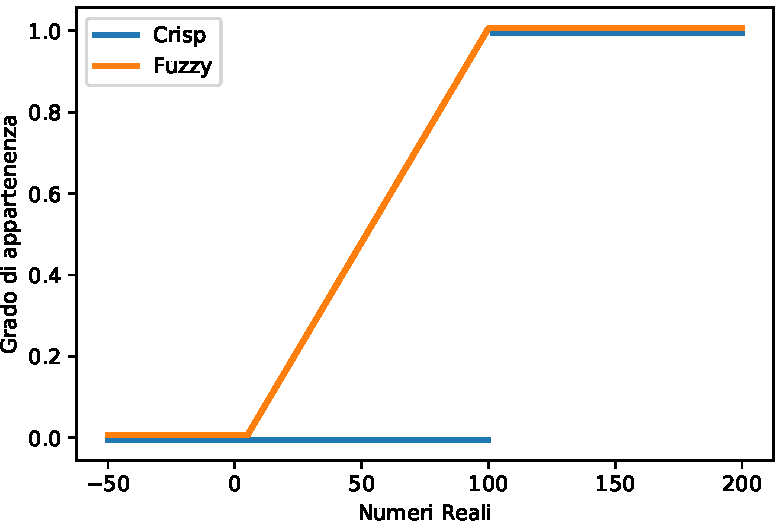
\includegraphics[scale=0.6]{figure/fuzzycrisp.pdf}
\caption{Grafico delle funzioni di appartenenza all'insieme ``Numeri molto più grandi di 1'' nelle versioni crisp e fuzzy \label{fuzzycrisp}}
\end{figure}che meglio rappresenta il concetto di \textit{molto} più grande alla base della definizione dell'insieme $A$. La \figurename~\ref{fuzzycrisp} mostra una rappresentazione grafica di questa funzione di appartenenza, sovrapposta a un'analoga rappresentazione del concetto di appartenenza per un insieme \textit{crisp}.\\
Nonostante l'appartenenza venga misurata con un numero compreso tra zero e uno, il concetto di appartenenza fuzzy non ha niente a che vedere con la probabilità che un elemento ha di appartenere a un certo insieme e la logica fuzzy non ha niente a che vedere con la probabilità che coinvolge variabili casuali e tratta di eventi e della loro possibilità di verificarsi. La \textit{fuzziness} è il risultato dell'imprecisione e dell'assenza di criteri chiari e ben definiti di appartenenza a un insieme.\\
Pertanto un insieme fuzzy è una collezione di oggetti con un grado non binario di appartenenza. Tale insieme è caratterizzato da una funzione che assegna a ogni oggetto un grado di appartenenza tra zero e uno, come formalmente indicato nella definizione seguente\cite{zadeh1965fuzzy}.
\begin{fuzzyset}
Sia $\Omega$ un insieme di punti in uno spazio, il cui generico elemento di $\Omega$ è denotato usando il simbolo $x$. Un \textit{insieme fuzzy} (o \textit{fuzzy set}) $A \subseteq \Omega$ è caratterizzato da una funzione di \textit{appartenenza} (o \textit{membership function}) $\mu_{A}(\cdot)$ che associa a ogni punto $x \in \Omega$ un valore reale nell'intervallo $[0,1]$, che rappresenta il \textit{grado di appartenenza} di $x$ a $A$.
\end{fuzzyset}
\begin{figure}[!h]
        \centering%
        \subfigure[Insieme delle persone giovani\label{giovani}]%
          {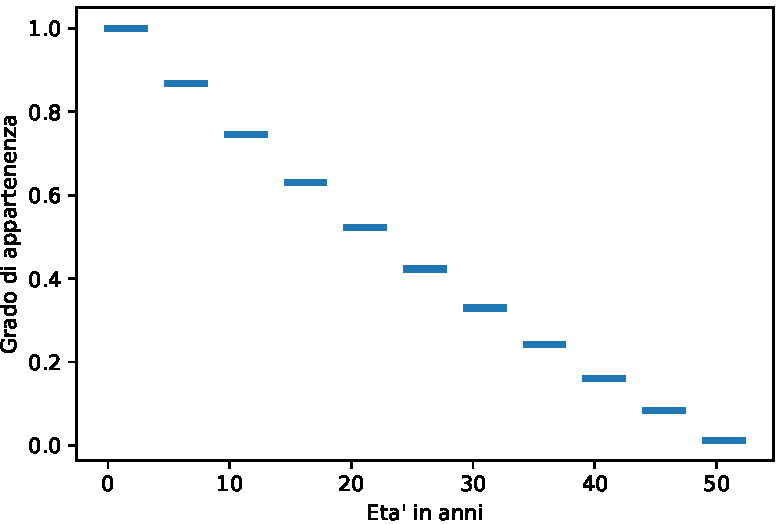
\includegraphics[scale=0.4]{figure/giovani.pdf}}\qquad\qquad
        \subfigure[Insieme delle bevande tiepide\label{tiepide}]%
          {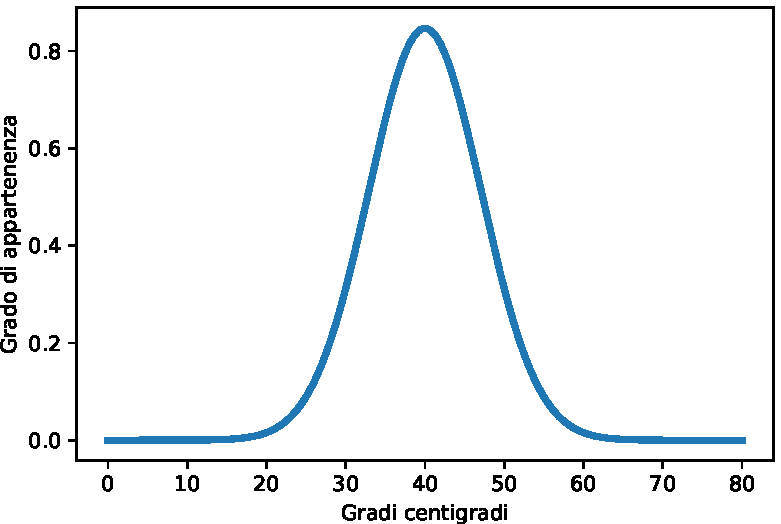
\includegraphics[scale=0.4]{figure/tiepide.pdf}}
          \caption{Alcuni esempi di fuzzy set con relativo grafico della funzione di appartenenza. Nella \figurename~\ref{giovani} l'insieme delle persone giovani è caratterizzato da una funzione costante a tratti e decrescente. Nella \figurename~\ref{tiepide} l'insieme delle bevande tiepide è caratterizzato da una funzione continua a campana.}
\end{figure}
\section{Operazioni tra insiemi fuzzy}
Sia per un insieme fuzzy, sia per un insieme del tipo ordinario, il grado di appartenenza zero ha il significato di \textit{non} appartenenza all'insieme e il grado di appartenenza 1 ha invece il significato di appartenenza. Gli insiemi fuzzy possono essere dunque visti come un'estensione degli insiemi crisp, mentre questi ultimi come un caso particolare di insiemi fuzzy la cui funzione di appartenenza è di tipo binario. Tutte le operazioni che si possono compiere con gli insiemi crisp sono estendibili agli insiemi fuzzy e tutte le definizioni fuzzy sono riconducibili a quelle crisp. Di seguito sono passate in rassegna le principali operazioni che coinvolgono degli insiemi, descrivendo come queste possano essere estese agli insiemi fuzzy.\\\\
\textbf{Insieme vuoto.} Un insieme fuzzy $A$ è vuoto, scritto $A = \varnothing$, se e solo se
\begin{equation} \mu_A(x) = 0 \; \forall \; x \in \Omega.\end{equation} 
\textbf{Uguaglianza.} Due insiemi fuzzy $A$ e $B$ sono uguali, scritto come $A=B$, se e solo se
\begin{equation} \mu_A(x) = \mu_B(x) \; \forall \; x \in \Omega.\end{equation} 
\textbf{Sottoinsiemi.} Un insieme fuzzy $A$ è sottoinsieme di un insieme fuzzy $B$, scritto come $A \subseteq B$, se e solo se
\begin{equation} \mu_A(x) \leq \mu_B(x) \; \forall \; x \in \Omega.\end{equation} 
\textbf{Complemento.} Il complemento di un fuzzy set $A$ è il fuzzy set $\bar{A}$, la cui funzione di appartenenza $\mu_{\bar{A}}$ è tale che
\begin{equation} \mu_{\bar{A}}(x) = 1-\mu_A(x) \; \forall \; x \in \Omega.\end{equation} 
\textbf{Unione.} L'unione tra un insieme fuzzy $A$ e un insieme fuzzy $B$ è un insieme fuzzy $C$, scritto $C=A \cup B$, la cui funzione di appartenenza $\mu_C$ è tale che
\begin{equation}\label{unione} \mu_C(x) = \max[\mu_A(x), \mu_B(x)] \; \forall \; x \in \Omega \end{equation} 
\textbf{Intersezione.} L'intersezione tra un insieme fuzzy $A$ e un insieme fuzzy $B$ è un insieme fuzzy $C$, scritto $C=A \cap B$, la cui funzione di appartenenza $\mu_C$ è tale che
\begin{equation} \mu_C(x) = \min[f_A(x), f_B(x)] \; \forall \; x \in \Omega. \end{equation} 
\textbf{Disgiunzione.} Due insiemi fuzzy $A$ e $B$ sono disgiunti se
\begin{equation} A \cap B = \varnothing. \end{equation} 
Va notato come queste estensioni non siano necessariamente uniche. Per esempio l'unione $A \cup B$ si può definire come il \textit{più piccolo} insieme fuzzy $C$ che contiene sia $A$ che $B$. Viceversa l'intersezione $A \cap B$ può essere definita come il \textit{più grande} insieme fuzzy $C$ che è contenuto sia in $A$ che in $B$. In entrambi i casi gli operatori $\cup$ e $\cap$ sono associativi.
%è possibile aggiungere esempi con immagini se necessario%
\section{Insiemi fuzzy di tipo 2}
Come visto nel paragrafo precedente, un fuzzy set modella un insieme i cui confini non sono ben definiti o sono incerti. Non vi è nessuno tipo di incertezza invece riguardo al grado di appartenenza $\mu_A(x)$ di un elemento $x$ a un insieme $A$. Gli insiemi fuzzy caratterizzati da una funzione di appartenenza \textit{non} incerta sono definiti insiemi fuzzy di tipo 1. Al contrario, gli insiemi fuzzy di tipo 2 ammettono funzioni di appartenenza incerte\cite{mendel2002type}.
\begin{fuzzyset2}
Un insieme fuzzy di tipo 2 $A$ è caratterizzato da una funzione di appartenenza $\mu_A(x,u)$, con $x \in \Omega$ e $u \in J_x \subseteq [0,1]$. Come per i fuzzy set del tipo 1 vale sempre $0 \leq \mu_A(x,u) \leq 1$.
\end{fuzzyset2}
Il valore $u$ equivale al grado di appartenenza $\mu_A(x)$ di $x$ all'insieme fuzzy di tipo 1 $A$. Il risultato di una funzione di appartenenza di tipo 2 è l'incertezza su un un certo grado di membership $u$ per un dato elemento $x$. Quando questa incertezza viene meno un insieme fuzzy di tipo 2 si riduce a un insieme fuzzy di tipo 1. Viceversa gli insiemi fuzzy di tipo 2 sono un'estensione degli insiemi fuzzy di tipo 1 con l'aggiunta di un grado di incertezza.
\begin{figure}[!h]
        \centering%
        \subfigure[Grafico di una funzione di appartenenza di tipo 2\label{fuzzy11}]%
          {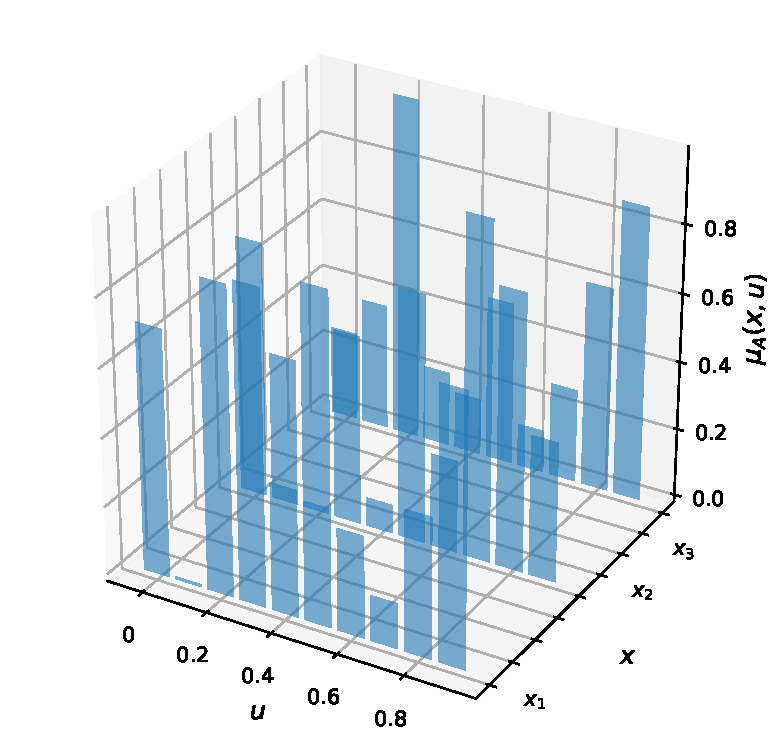
\includegraphics[scale=.45]{figure/fuzzy11.pdf}}\qquad\qquad
        \subfigure[Ad ogni valore $x \in \Omega$ corrisponde un piano i cui assi sono $u$ e $\mu_A(x,u)$. In evidenza il piano corrispondente a $x_1$\label{fuzzy12}]%
          {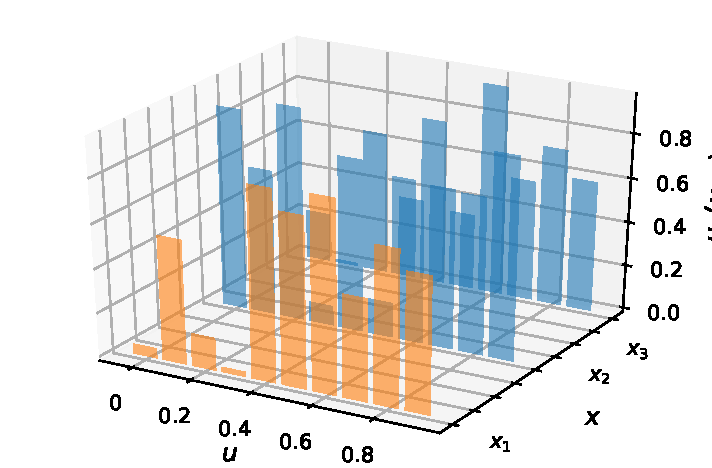
\includegraphics[scale=.45]{figure/fuzzy12.pdf}}
          \caption{Insiemi fuzzy di tipo 2.}
\end{figure}
\chapter{Le support vector machine}
\section{Classificazione}
Classificare significa assegnare oggetti a classi secondo criteri di affinità. Un problema di classificazione consiste nella costruzione di una regola $f: \Omega \rightarrow Y$ che associa gli elementi del dominio $\Omega$ alle \textit{etichette} appartenenti al codominio $Y$ dove ogni diversa etichetta individua una diversa classe. L'insieme $\Omega$ tipicamente è un sottoinsieme $\Omega \subseteq \mathbb{R}^d$. Il generico elemento di $\Omega$ è quindi un punto \textit{d}-dimensionale. Ciascuna delle \textit{d} dimensioni equivale a una specifica \textit{feature} della famiglia di oggetti $\Omega$. Nell'ambito del machine-learning il processo di costruzione della regola $f$ è detto \textit{apprendimento}. Durante la fase di apprendimento , un algoritmo visiona un insieme di esempi $T=\lbrace (x_0,y_0), (x_1,y_1), \cdots, (x_n,y_n) \rbrace$, dove la generica coppia $(x_i,y_i)$, con $x_i \in X \subseteq \Omega$ e $y_i \in Y$, è un esempio di classificazione corretta di $x_i$ con l'etichetta $y_i$, e ne estrae un criterio di classificazione generale per tutti i punti appartenenti a $\Omega$, cioè la funzione $f(\cdot)$. L'insieme $T$ prende il nome di \textit{training set}.\\
La notazione $x_i$ indica il primo elemento della \textit{i}-esima coppia appartenente a un training set. Mentre la notazione $x_{i}^{(j)}$ indica la \textit{j}-esima componente del vettore $x_i$. Quando la cardinalità dell'insieme di arrivo è $|Y|=2$, si parla di classificazione binaria. Per comodità di notazione e di calcolo da qui in poi verranno presentati esempi di classificazione binaria in cui l'insieme $Y$ delle possibili etichette è $Y=\lbrace-1,1\rbrace$.
\subsection{Percettrone}
Il percettrone\cite{rosenblatt1958perceptron} è un classificatore binario a soglia che assegna un oggetto $x \in \Omega$ alla classe ottenuta utilizzando la seguente regola:
\begin{equation}
f_P(x)=
\begin{cases}
+1 & \textit{se } w \boldsymbol{\cdot} x \geq \theta, \\
-1 & \textit{se } w \boldsymbol{\cdot} x < \theta,
\end{cases}
\end{equation}
dove $w$ è un vettore di pesi delle stesse dimensioni del vettore di input $x$, $\theta$ è la soglia discriminante nella classificazione di un punto, ilsimbolo $\boldsymbol{\cdot}$ indica il prodotto scalare. Se la somma delle componenti del vettore input $x$ pesate secondo quelle del vettore $w$ supera una certa soglia $\theta$, il percettrone dà un responso \textit{positivo}, altrimenti \textit{negativo}. L'iperpiano di equazione $w \boldsymbol{\cdot} x = \theta$ separa in $\Omega$ la classe positiva da quella negativa. La classificazione tramite percettrone è quindi applicabile a classi \textit{linearmente separabili} nello spazio di definizione. La fase di apprendimento dell' iperpiano separatore $w^* \boldsymbol{\cdot} x = \theta$ consiste nell'aggiustare iterativamente i valori di $w$ fino a quando non si ottiene un iperpiano separatore corretto per il training set visionato, secondo una procedura simile a quella descritta nell'Algoritmo \ref{iperpiano}.
\begin{algorithm}
\caption{Ricerca dell'iperpiano separatore}\label{iperpiano}
\begin{algorithmic}[1]
\State inizializzare $w$ con un vettore casuale
\While{esistono errori di classificazione}
	\State $i=0$
	\While{$i<|T|$}
		\State $y' = w \boldsymbol{\cdot} x_i - \theta$
		\If{$y' \cdot y < 0$} $w = w + \eta y x_i$ \EndIf
	\EndWhile
\EndWhile
\end{algorithmic}
\end{algorithm}
Si può dimostrare\cite{rosenblatt1958perceptron} che quando le due classi sono linearmente separabili, il Punto 9.\ viene superato dopo un numero finito di iterazioni. In tal caso, l'iperpiano separatore è individuato da $w^* \boldsymbol{ \cdot} x = \theta$, dove $w^*$ è il valore di $w$ al termine dell'esecuzione dell'Algoitmo \ref{iperpiano}. In presenza di classi \textit{non} linearmente separabili il precedente algoritmo rimane bloccato in un loop infinito.  L'Istruzione 5.\ esegue l'aggiornamento di $w$, facendo in modo che il nuovo $w$ risulti spostato verso il vettore $x_i$ che è mal classificato in quel momento. Il parametro $\eta > 0$ definisce la misura dello spostamento e di conseguenza la velocità con cui $w$ si avvicina alla soluzione. Un $\eta$ troppo grande potrebbe portare a una situazione di loop infinito in cui $w$ continua ad aggiornarsi tra due valori, uno più grande, uno più piccolo della soluzione, o anche a far divergere $w$. Nell'Algoritmo \ref{iperpiano} la soglia $\theta$ è trattata come costante. È possibile permettere alla soglia di variare eliminandola di fatto dalla formalizzazione e aggiungendo una variabile in coda, come nuova dimensione, al vettore $w$. Aggiungendo agli esempi $x_i$ con lo stesso metodo il peso -1 il calcolo di $y'$ risulta analogo a quello del punto 3 e la soglia è in grado di variare come ogni altra singola componente di $w$. Accettando di avere a che fare con classi non separabili l'algoritmo può essere modificato permettendo lo stop secondo alcuni criteri, per esempio eseguendo un numero fissato di cicli, oppure fermandosi quando il numero di classificazioni errate smette di variare al variare di $w$.
\subsection{Macchine a vettori di supporto}
Una macchina a vettori di supporto\cite{cortes1995support}, \textit{support vector machine}, o SVM in breve, ha come scopo non solo quello di trovare un iperpiano $w \boldsymbol{\cdot} x + b = 0$ che separi linearmente i dati, ma anche di fare in modo che l'iperpiano minimizzi l'errore durante la fase di classificazione di punti al di fuori dell'insieme di training. Questo iperpiano è quello posizionato alla stessa distanza da entrambe le classi. La distanza di una classe da un piano equivale alla minima distanza punto-piano misurata per ogni punto appartenente alla classe. Questa distanza viene definita \textit{margine}. Utilizzare l'iperpiano equidistante dalle classi per la discriminazione tra le due permette di massimizzare il margine e ottenere così una migliore generalizzazione, cioè una migliore capacità di classificare correttamente anche punti non presenti nel training set. In  \figurename~\ref{margine} la rappresentazione grafica di quanto descritto finora.
\begin{figure}[!h]
\centering
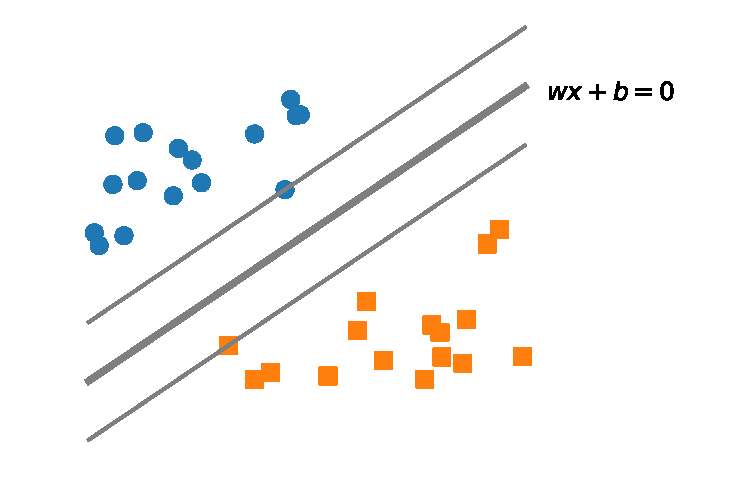
\includegraphics[scale=.6]{figure/margine.pdf}
\caption{Iperpiano separatore per due classi linearmente separabili in due dimensioni. Il margine equvale alla distanza tra la retta di equazione $wx + b = 0$ e le due rette più sottili.\label{margine}}
\end{figure}\\
La fase di apprendimento di SVM consiste nella massimizzazione del margine $\gamma$, variando i parametri $w$ e $b$, soggetta al vincolo che per ogni punto $x_i$ valga
\begin{equation}
y_i(w\boldsymbol{\cdot}x_i + b) \geq \gamma.
\end{equation}
Indicando con $w^*$ e $b^*$ le soluzioni del precedente problema di massimizzazione sono individuati
\begin{itemize}
\item[]$w \boldsymbol{\cdot} x + b = 0$, l'iperpiano separatore.
\item[]$w \boldsymbol{\cdot} x + b = \gamma$, il confine della classe positiva.
\item[]$w \boldsymbol{\cdot} x + b = -\gamma$, il confine della classe negativa.
\end{itemize}
I punti che soddisfano l'equazione $w^* \boldsymbol{\cdot} x + b^* = \pm \gamma$, si trovano esattamente a distanza $\gamma$ dal separatore e si trovano sul confine delle loro classi. Tali punti prendono il nome di \textit{support vector} o \textit{vettori di supporto}. La  \figurename~\ref{supportvector} mette in evidenza i vettori di supporto per due classi linearmente separabili.
\begin{figure}[!h]
\centering
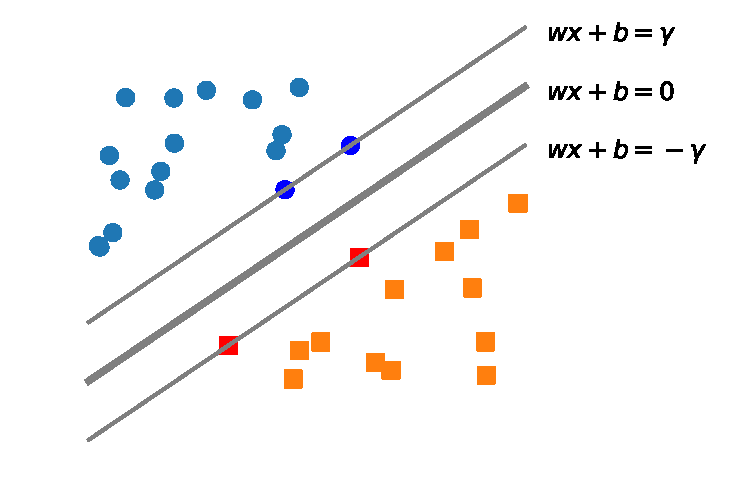
\includegraphics[scale=.6]{figure/supportvectors.pdf}
\caption{Vettori di supporto per due classi di punti linearmente separabili.\label{supportvector}}
\end{figure}Scelta una coppia $(w^*, b^*)$ di soluzioni, è sempre possibile trovare una coppia $(kw^*, kb^*)$, per $k>1$, anch'essa soluzione, per cui è sempre vero che $k\gamma > \gamma$. In altre parole, $\gamma$ non può essere massimizzato. La soluzione a questo problema consiste nella normalizzazione del vettore $w$ costringendo $\gamma$ a essere multiplo del vettore unità $\dfrac{w}{\parallel w \parallel}$. Questo cambia il problema di ottimizzazione nella minimizzazione di $\parallel w \parallel$ soggetta al vincolo che per ogni punto $x_i$ valga
\begin{equation}
y_i(w\boldsymbol{\cdot}x_i + b) \geq 1.
\end{equation}
Una volta determinati tali valori ottimali, la classificazione viene eseguita secondo la regola
\begin{equation}\label{fsvm}
f_\mathrm{SVC}(x)=
\begin{cases}
+1 & \textit{se } w^* \boldsymbol{\cdot} x + b^* \geq 0, \\
-1 & \textit{se } w^* \boldsymbol{\cdot} x  + b^*< 0.
\end{cases}
\end{equation}
Va notato che il problema di minimizzazione di $\parallel w \parallel$ e quello di una qualsiasi funzione monotona di $\parallel w \parallel$ hanno le stesse soluzioni. Per comodità di derivazione e risoluzione normalmente si sceglie di costruire il problema di minimizzazione attorno alla funzione $f(\parallel w \parallel) = \dfrac{1}{2}\parallel w \parallel ^2$, trasformando il problema nel minimizzare $\dfrac{1}{2}\parallel w \parallel ^2$ soggetta ai vincoli $ y_i(w\boldsymbol{\cdot}x_i + b) \geq 1 \; \forall \; x_i \in X$. Scrivere la lagrangiana
\begin{equation}
\label{lagrange}
L = \dfrac{1}{2}\parallel w\parallel ^2 - \sum_{i=1}^n \alpha_i [y_i(w \boldsymbol{\cdot} x_i +b -1)],
\end{equation}
dove ogni $\alpha_i \geq 0$ è un moltiplicatore lagrangiano, permette di inglobare i vincoli nel problema. Differenziando $L$ rispetto a $w$, e rispetto a $b$ poi, e ponendo tali derivate uguali a zero, si ottiene
\begin{itemize}
\item[]\begin{equation}\label{w}
\dfrac{{\partial L}}{{\partial w}} = 0 \Longrightarrow w = \sum_{i=1}^n \alpha_i y_i x_i,
\end{equation}
\item[]\begin{equation}\label{b}\dfrac{\partial L}{\partial b} = 0 \Longrightarrow \sum_{i=1}^n \alpha_i y_i = 0.
\end{equation}
\end{itemize}
Questi risultati, sostituiti in \eqref{lagrange}, portano a quello che è definito \textit{problema duale}\cite{fletcher1987practical}: massimizzare, variando le nuove variabili $\alpha_i$,
\begin{equation}\label{duale}
L_D = \sum_{i=1}^n \alpha_i -\dfrac{1}{2} \sum_{i,j}^n \alpha_i \alpha_j y_i y_j x_i \boldsymbol{\cdot} x_j
\end{equation}
soggetta ai vincoli
\begin{equation}
\alpha_i \geq 0 \; \forall i \in \lbrace 1, \cdots n \rbrace,
\end{equation}
\begin{equation}
\sum_{i=1}^n \alpha_i y_i = 0.
\end{equation}
Inoltre, per le condizioni di Karush-Kuhn-Tucker\cite{kuhn1951proceedings} (condizioni KKT), deve valere per ogni $i \in \lbrace 1, \cdots, n \rbrace$ 
\begin{equation}
\alpha_i[y_i(w \boldsymbol{\cdot} + b -1)] = 0.
\end{equation}
Risulta quindi che per le soluzioni $\alpha_i^* > 0$ del problema duale è soddisfatta l'uguaglianza $y_i(w \boldsymbol{\cdot} x_i + b) = 1$. Di conseguenza $x_i$ è un vettore di supporto e $w^*$ è ricavabile da (\refeq{w}), come combinazione lineare dei vettori di supporto. Mentre $b^*$ è la soluzione dell'equazione $y_i(w^* \boldsymbol{\cdot} x_s + b)= 1$ dove $x_s$ è uno tra i vettori di supporto individuati.
\subsection{Kernel Trick}
Quello di utilizzare uno, o più, piani separatori è un buon metodo di classificazione in presenza di dati linearmente separabili. Al contrario, in presenza di dati non linearmente separabili, qualsiasi scelta per la coppia $(w^*, b^*)$ produce un iperpiano che mal classifica almeno un elemento del training set. La  \figurename~\ref{nonseparabili} rappresenta graficamente una di queste situazioni.\\
\begin{figure}[!h]
\centering
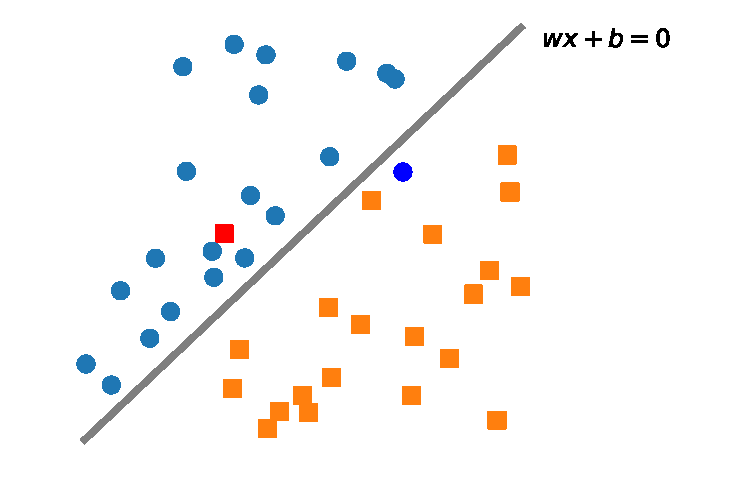
\includegraphics[scale=.6]{figure/nonseparabili.pdf}
\caption{Esempio in due dimensioni di classi non linearmente separabili. In evidenza i punti male classificati. \label{nonseparabili}}
\end{figure}Una delle possibili soluzioni è quella di trasformare i dati in modo che risultino essere linearmente separabili utilizzando il \textit{kernel trick}. L'idea che sta dietro al \textit{trucco} è quella che punti \textit{d}-dimensionali, non linearmente separabili in \textit{d} dimensioni, potrebbero esserlo se trasportati in uno spazio a maggiore dimensionalità. Una funzione $\phi: \mathbb{R}^d \rightarrow \mathbb{R}^D$, per $D > d$, che trasporta punti in uno spazio a maggiore dimensionalità aggiungendo le feature mancanti come funzione di quelle originali è chiamata \textit{mapping}. Il codominio di un mapping invece prende il nome di \textit{spazio delle feature}. Per sortire l'effetto di produrre dati linearmente separabili un mapping deve poter proiettare in porzioni differenti dello spazio punti appartenenti a differenti classi.\\\\
\textbf{Esempio 1.} Dato il training set $T_1=\lbrace (1,a),(-2,a),(3,b),(-3,b),(-4,b), \linebreak (-1,a),(4,b),(2,a) \rbrace$ dove $X = \lbrace x \in \mathbb{N} | -5 < x < 5 \rbrace$ e $Y=\lbrace a,b \rbrace$. Le due differenti classi risultano non linearmente separabili sulla retta dei reali [\figurename~\ref{mapping12}]. Il mapping $\phi_1(x)=(x,x^2)$ proietta verso l'alto gli $x \in X$ con modulo maggiore, rendendo il training set linearmente separabile nelle due dimensioni (\figurename~\ref{mapping12}).\\\\
\textbf{Esempio 2.} Dato il training set $T_2=\lbrace [(0;3),a], [(3;0),a], [(1;2),b], (2;1),b], \linebreak (3/2;0),a], [(0;3/2),a], [(1;1),b], [(2;2),b], [(0;0),a], [(3/2; 3/2)] \rbrace$, con $X \subset \mathbb{R}^2$. Le classi $a, b \in Y$ non sono linearmente separabili [\figurename~\ref{mapping21}]. La trasformazione $\phi_2(x,y)=(x,y,xy)$ produce valori bassi nella terza dimensione per i punti etichettati $a$, valori alti per i punti etichettati $b$, rendendo l'immagine di $X$ linearmente separabile nello spazio tridimensionale [\figurename~\ref{mapping22}].\\\\
In questo caso la regola di classificazione diventa quindi
\begin{equation}
f_K(x)=
\begin{cases}
+1 & \textit{se } w^* \boldsymbol{\cdot} \phi(x) + b^* \geq 0, \\
-1 & \textit{se } w^* \boldsymbol{\cdot} \phi(x)  + b^*< 0.
\end{cases}
\end{equation}
La denominazione \textit{kernel trick} deriva dal fatto che il trucco è utilizzato in coppia con funzioni denominate \textit{kernel function}\cite{shawe2004kernel}. Considerato un mapping $\phi$, una kernel function $K$ è definita in modo tale che sia sempre valido
\begin{equation}
K(x_i,x_j) = \phi(x_i) \boldsymbol{\cdot} \phi{x_j}.
\end{equation}
In questo modo, conoscendo $K$, è possibile calcolare il prodotto scalare tra due elementi nello spazio delle feature senza dover effettivamente calcolare i mapping corrispondenti. Così facendo la (\refeq{duale}) può essere riscritta in questo modo:
\begin{equation}
L_D = \sum_{i=1}^n \alpha_i -\dfrac{1}{2} \sum_{i,j}^n \alpha_i \alpha_j y_i y_j K(x_i,x_j).
\end{equation}
\begin{figure}[!h]
        \centering%
         \subfigure[Training set $T_1$ in $\mathbb{R}$\label{mapping11}]%
          {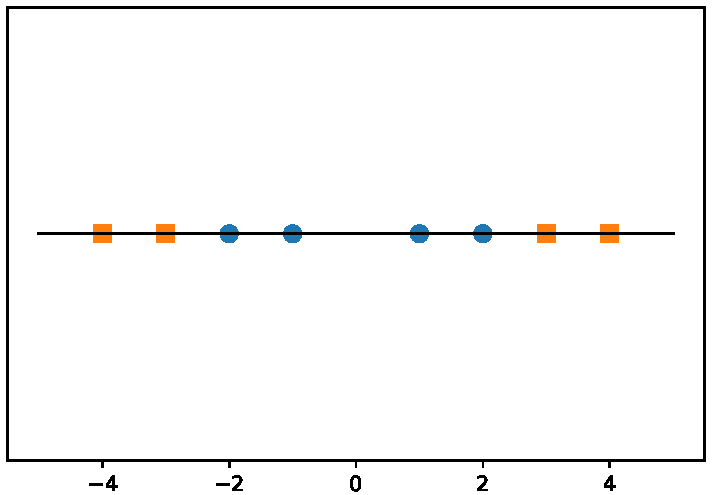
\includegraphics[scale=0.4]{figure/mapping11.pdf}}\qquad\qquad
        \subfigure[Training set $T_2$ mappato in $\mathbb{R}^2$ da $\phi_1$\label{mapping12}]%
          {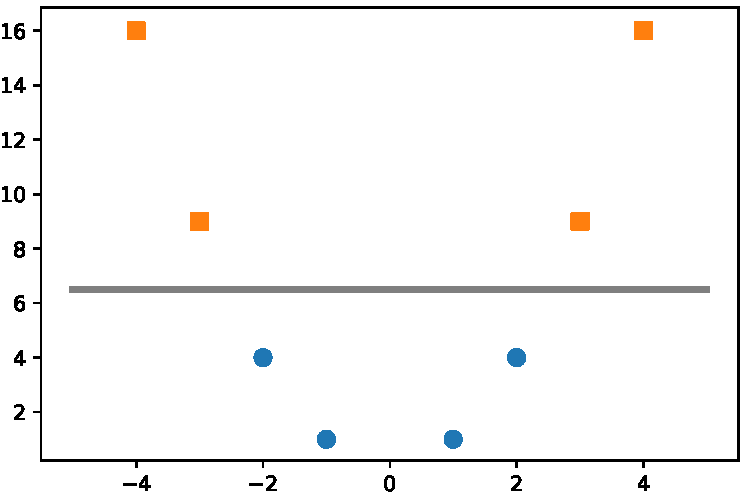
\includegraphics[scale=0.4]{figure/mapping12.pdf}}\qquad\qquad
        \subfigure[Training set $T_2$ in $\mathbb{R}^2$\label{mapping21}]%
          {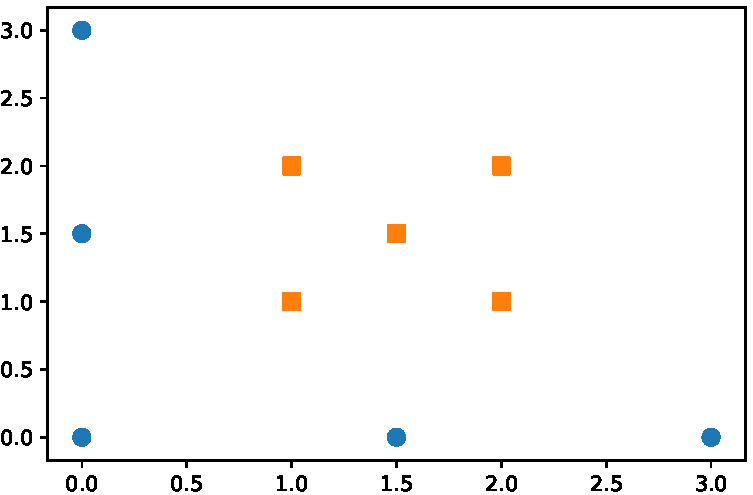
\includegraphics[scale=0.4]{figure/mapping21.pdf}}\qquad\qquad
        \subfigure[Training set $T_2$ mappato in $\mathbb{R}^3$ da $\phi_2$\label{mapping22}]%
          {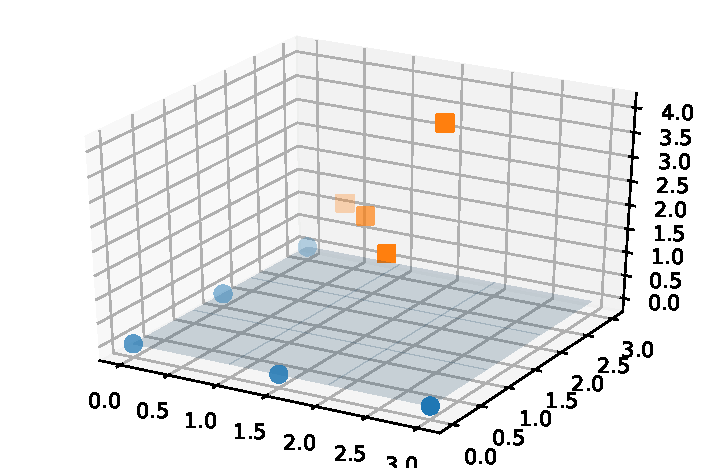
\includegraphics[scale=0.4]{figure/mapping22.pdf}}
          \caption{Training set degli esempi 1 e 2. A sinistra nello spazio originale, a destra dopo la trasformazione in più dimensioni.}
\end{figure}\linebreak
Nei capitoli successivi ogniqualvolta si fa riferimento a una funzione kernel si intende una funzione kernel di tipo gaussiano\cite{vert2004primer} così definita:
\begin{equation}
\phi(x) = e^{-\dfrac{x^2}{2\sigma^2}} [1, \sqrt{\dfrac{1}{1! \sigma^2}}x, \sqrt{\dfrac{1}{2! \sigma^4}}x^2, \sqrt{\dfrac{1}{3!\sigma^6}}x^3, \cdots]^T.
\end{equation}
La particolarità del kernel gaussiano è quella di mappare punti in un insieme con infinite dimensioni. Il risultato del prodotto scalare $\phi(x_i) \boldsymbol{\cdot} \phi(x_j)$ risulta invece essere
\begin{equation}
K(x_i,x_j) = e^{-\dfrac{\parallel x_i - x_j \parallel^2}{2\sigma^2}}.
\end{equation}
\subsection{Dati non linearmente separabili}
L'utilizzo del kernel trick non è sempre garanzia di separazione lineare delle classi. Inoltre in alcune situazioni lasciare che i dati siano non separabili è funzionale alla risoluzione del problema di classificazione. Anche in questo caso nessuna coppia $(w^*,b^*)$ individua un iperpiano che non commette errori di classificazione. Non potendo essere eliminati totalmente, gli errori di classificazione diventano parte integrante della ricerca del criterio di classificazione. Il migliore iperpiano apprendibile da un training set diventa allora quello che commette il minor numero di errori, o gli errori più veniali, e si mantiene sufficientemente lontano dai confini delle classi. Un iperpiano incorre in una penalità ogniqualvolta classifichi in modo errato un punto o gli si avvicini a una distanza minore di un certo $\gamma$. I punti classificati correttamente ma troppo vicini al piano vengono definiti \textit{outliers}(\figurename~\ref{outliers}). Ogni penalità è pesata in base alla distanza del punto dall'iperpiano. Il piano che minimizza l'ammontare $l(w,b)$ della penalità è quello poi utilizzato per classificare i punti al di fuori del training set.
\begin{equation}
l(w,b)= \dfrac{1}{2} \sum_{j=1}^d w^{(j)^2} + C \sum_{i=1}^n \max[0, 1 - y_i(\sum_{j=1}^d w^{(j)} x_i^{(j)} + b)].
\end{equation}
Il primo termine di $l(w,b)$, al fine di normalizzare $\parallel w \parallel ^2$ come visto nel Paragrafo 2.1.2, favorisce $w$ composti da piccole componenti. Il parametro di \textit{tradeoff} $C > 0$ indica quanto l'ammonatare della penalità pesa rispetto al precedente addendo. Valori bassi di $C$ ammettono più errori di classificazione ma allargano i margini tra iperpiano e classi, mentre valori alti di $C$ ammettono meno errori di classificazione ma diminuiscono i margini.
\begin{figure}[H]
\centering
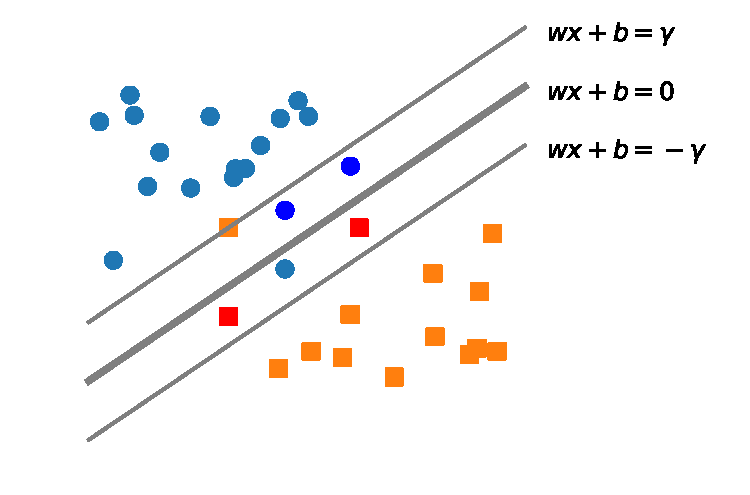
\includegraphics[scale=.7]{figure/outliers.pdf}
\caption{In evidenza gli outliers per un insieme di punti bidimensionali. Nel grafico sono presenti anche due errori di classificazione. \label{outliers}}
\end{figure}
\noindent
Anche in questa situazione il criterio di classificazione è dato dalla
\begin{equation}
f_\mathrm{SVC}(x)=
\begin{cases}
+1 & \textit{se } w^* \boldsymbol{\cdot} x + b^* \geq 0, \\
-1 & \textit{se } w^* \boldsymbol{\cdot} x  + b^*< 0.
\end{cases}
\end{equation}
che differisce dalla \refeq{fsvm} per il metodo di training dell'iperpiano $w^* \boldsymbol{\cdot} x + b^* = 0$.
È utile notare che allo stesso modo che per (\refeq{lagrange}) è possibile ricavare il problema duale alla minimizzazione di $l(w,b)$, e cioè massimizzare
\begin{equation}\label{lossduale}
l_D = \sum_{i=1}^n \alpha_i -\dfrac{1}{2} \sum_{i,j}^n \alpha_i \alpha_j y_i y_j x_i \boldsymbol{\cdot} x_j
\end{equation}
soggetta ai vincoli
\begin{equation}
0 \leq \alpha_i \leq C \: \forall \: i \in \lbrace 1, \cdots n \rbrace.
\end{equation}
Infine, gli approcci proposti finora possono essere mescolati, come è il caso del problema denominato 1-SVM affrontato nel prossimo paragrafo.
\section{1-SVM}
1-SVM è un particolare caso di classificazione mediante macchine a vettori di supporto in cui il numero di classi presenti nel problema è pari a uno. Distribuire punti all'interno di una singola classe non significa costruire una funzione che restituisce l'unica possibile etichetta per ogni possibile valore di input, ma racchiudere all'interno di una porzione di spazio più piccola possibile il maggior numero di punti di un training set, ammettendo alcuni outliers. Ciò permette successivamente di rilevare per esempio dei dati anomali. Formalmente, dato un insieme di oggetti $X = \lbrace x_1, x_2, \cdots, x_n \rbrace$, $X \subseteq \mathbb{R}^d$, e un mapping $\phi: \mathbb{R}^d \rightarrow \mathbb{R}^D$, con $D > d$, il problema di classificazione 1-SVM si riconduce alla ricerca nello spazio $\mathbb{R}^D$ della più piccola (\textit{iper})sfera di raggio $R$ e centro $a$ che racchiuda in sé la maggior parte dei punti appartenenti all'insieme $X$. Ciò equivale a minimizzare $R$ sotto il vincolo che per ogni $x_i \in X$ valga
\begin{equation}\label{sfera}
\parallel \phi(x_i) - a \parallel^2 \leq R^2 + \xi_i,
\end{equation}
dove $\xi_i > 0 \; \forall \; i \in \lbrace 1, \cdots, n \rbrace$  sono variabil slack.\\
Analogamente a quanto visto nel Paragrafo 2.1.4 il problema di minimizzazione viene risolto introducendo una funzione lagrangiana:
\begin{equation}
L = R^2 - \sum_{i=1}^n (R^2 + \xi_i - \parallel \phi(x_i) - a \parallel^2) \beta_i - \sum_{i=1}^n \xi_i \mu_i + C \sum_{i=1}^n \xi_i.
\end{equation}
Il primo addendo regola la misura del raggio, la prima sommatoria l'ampiezza dei margini tra la superficie della sfera e gli outlier, il termine $\sum_{i=1}^n\xi_i$ è un termine di penalità pesato per il parametro $C$. Mentre $\beta_i$ e $\mu_i$ sono moltiplicatori lagrangiani. Ponendo uguale a zero la derivata di $L$ questa volta rispetto a $R$, $a$ e $xi_i$ si ottiene
\begin{equation}\label{beta}
\sum_{i=1}^n \beta_i = 1,
\end{equation}
\begin{equation}\label{centro}
a = \sum_{i=1}^n \beta_i \phi(x_i),
\end{equation}
\begin{equation}\label{C}
\beta_i = C - \mu_i.
\end{equation}
Inoltre devono valere per ogni $i \in \lbrace 1, \cdots, n \rbrace$ le condizioni KKT
\begin{equation}\label{kkt1}
\xi_i\mu_i = 0,
\end{equation}
\begin{equation}\label{kkt2}
(R^2 + \xi_i - \parallel \phi(x_i)-a \parallel^2 \beta_i = 0).
\end{equation}
Segue dalla (\refeq{kkt2}) che l'immagine di un punto $x_i$ a cui corrispondono $\xi_i > 0$ e $\beta_i > 0$ risiede al di fuori della sfera. Inoltre, essendo $\xi_i = 0$, per la condizione (\refeq{kkt1}), al punto $x_i$ deve anche corrispondere $\mu_i$ tale che $\mu_i = 0$. Conseguentemente, per la (\refeq{C}), risulta $\beta_i = C$. Se invece, $\beta_i$ è tale che $0 < \beta_i < C$, per la (\refeq{kkt2}), gli $x_i$ corrispondenti sono mappati sulla superficie della sfera. Da quanto appena dimostrato consegue che ogni $\beta_i^*$, soluzione del problema di ottimizzazione, permette di classificare il corrispondente oggetto $x_i$ nel modo descritto di seguito.
\begin{itemize}
\item Se $\beta_i^*=0$ l'immagine di $x_i$ secondo $\phi$ si trova all'interno della sfera.
\item Se $0 < \beta_i^* < C$ l'immagine di $x_i$ secondo $\phi$ si trova sulla superficie della sfera e $x_i$ è un vettore di supporto.
\item Se $\beta_i^*=C$ l'immagine di $x_i$ è mappata al di fuori della sfera e $x_i$ è considerato un outlier.
\end{itemize}
Successivamente, in modo simile a come visto per (\refeq{duale}) e per (\refeq{lossduale}), è possibile riscrivere il problema in forma duale di Wolfe\cite{wolfe1961duality}: dal problema vengono eliminate le variabili $R$, $a$ ed $\mu_i$, ottenendo il nuovo obiettivo
\begin{equation}
W = \beta_i\sum_{i=1}^n\phi(x_i)^2 - \sum_{i=1}^n\sum_{j=1}^n\beta_i\beta_j\phi(x_i)\boldsymbol{\cdot}\phi(x_j),
\end{equation}
da ottimizzare rispettando i vincoli
\begin{equation}
0 < \beta_i \leq C \; \forall \; i \in \lbrace 1, \cdots, n \rbrace.
\end{equation}
Infine il prodotto scalare $\phi(x_i)$ può essere riscritto mediante l'utilizzo di una \textit{kernel function}, ottenendo
\begin{equation}
W = \sum_{i=1}^n\beta_iK(x_i,x_i) - \sum_{i=1}^n\sum_{j=1}^n\beta_i\beta_jK(x_i,x_j).
\end{equation}
A classificazione avvenuta il raggio $R$ risulta essere uguale alla distanza dal centro di uno dei vettori di supporto individuati. Il quadrato della distanza di un generico punto $x$ dal centro della sfera invece può essere calcolata in virtù di (\refeq{centro}) mediante
\begin{equation}\label{r}
R^2(x) = K(x,x) - 2 \sum_{i=1}^n \beta_i K(x_i,x) + \sum_{i=1}^n\sum_{j=1}^n\beta_i\beta_jK(x_i,x_j).
\end{equation}
\section{Clustering}
È possibile utilizzare 1-SVM per la risoluzione di problemi di clustering. Dopo aver applicato il procedimento descritto nel paragrafo precedente a un insieme di punti $a \in A \subseteq \mathbb{R}^d$, si dispone di una sfera che ingloba la maggior parte delle immagini $\phi(a)$ nello spazio delle feature e di una funzione $R^2(\cdot)$ che permette di calcolare il quadrato della distanza di una generica immagine $\phi(x)$ dal centro della sfera che rende così noto anche il raggio $R$. Conoscendo queste informazioni è possibile costruire un metodo per la divisione dei punti $a \in A$ in diversi cluster\cite{ben2001support}. Due punti sono considerati appartenere allo stesso cluster se ogni punto del segmento che li unisce è mappato da $\phi$ all'interno della sfera, cioè risulti $R^2(p) \leq R^2$ per ogni punto $p$ del segmento. Costruendo un grafo avente come nodi tutti i possibili $a \in A$ e tracciando un arco tra il nodo \textit{i} ed  il nodo \textit{j} solo se il segmento che congiunge $a_i$ con $a_j$ è interamente mappato all'interno della sfera, le diverse componenti connesse del grafo corrispondono ai vari cluster in cui $A$ è diviso. Questo metodo di divisione in cluster mediante 1-SVM è definito \textit{support vector clustering}.
\begin{figure}[H]
        \centering%
        \subfigure[Due coppie di punti collegate da un segmento in uno spazio bidimensionale.\label{clustering11}]%
          {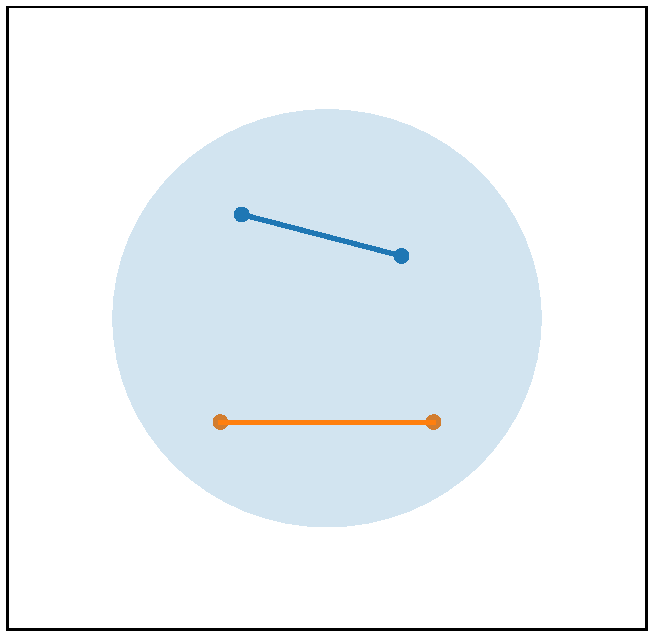
\includegraphics[scale=.35]{figure/clustering11.pdf}}\qquad\qquad
        \subfigure[Coppie di punti collegate da un segmento in uno spazio tridimensionale.\label{clustering12}]%
          {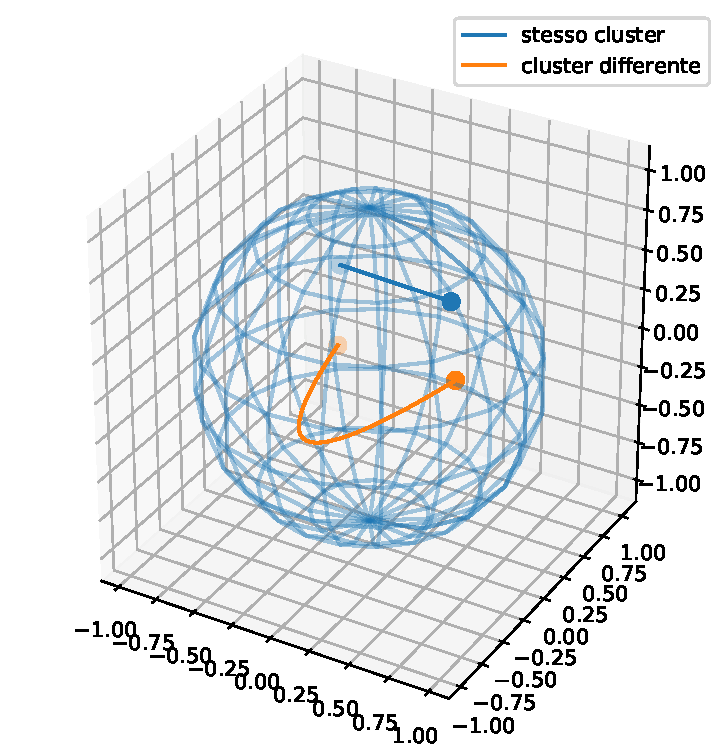
\includegraphics[scale=.35]{figure/clustering12.pdf}}
          \caption{Metodo di clustering 1-SVM. In \figurename~\ref{clustering11} due coppie di punti in uno spazio bidimensionale. In \figurename~\ref{clustering12} le stesse coppie di punti mappate in uno spazio tridimensionale. Si noti come l'immagine del segmento congiungente i due punti non appartenenti allo stesso cluster esca dalla sfera soluzione di 1-SVM.}
\end{figure}
\chapter{Apprendimento di insiemi fuzzy}\label{malchiodi}
Come visto in precedenza, un insieme fuzzy è definito dalla sua funzione di appartenenza. Un algortimo di apprendimento per insiemi fuzzy di conseguenza deve essere costruito in modo tale che l'elaborazione delle informazioni presenti nel training set conduca alla costruzione di una funzione di appartenenza.
Sia $X=\lbrace x_1, x_2, \cdots, x_n \rbrace \subset \Omega$ un insieme di punti \textit{d}-dimensionali e $U=\lbrace \mu_1, \mu_2, \cdots, \mu_n \rbrace$ un insieme di gradi di appartenenza a un insieme fuzzy ignoto $A$, tale che $\mu_i$ è il grado di appartenenza di $x_i$ a $A$. Apprendere l'insieme fuzzy $A$ significa costruirne la funzione di appartenenza $\mu_A(\cdot)$ visionando gli insiemi di training $X$ e $U$. Questo problema\cite{malchiodi2013learning} consiste in due fasi: la ricerca dei confini dell'insieme fuzzy e la costruzione della sua funzione di appartenenza.
\section{Ricerca dei confini}
Come visto in precedenza, i confini di un insieme fuzzy non sono una linea di demarcazione netta tra i punti appartenenti all'insieme e quelli che invece non vi appartengono. La ricerca dei confini di un insieme fuzzy $A$ consiste in realtà nella ricerca di un sottoinsieme $X_c \subseteq X$ a cui assegnare la proprietà $x \in X_c \rightarrow \mu_A(x) = 1$. L'insieme $X_c$ così definito prende il nome di \textit{core}. L'insieme fuzzy che ne risulta è quindi composto da un insieme di punti racchiusi all'interno di confini netti e da altri che invece giacciono al di fuori di essi, come è il caso degli outliers dell'algoritmo 1-SVM. Il problema (\refeq{sfera}) di ricerca della più piccola sfera di raggio $R$ e centro $a$ è modificato in modo tale da racchiudere il \textit{core} dell'insieme fuzzy $A$ all'interno della sfera tenendo conto del grado di appartenenza di ciascun punto del training set. Il problema modificato consiste nel minimizzare
\begin{equation}
R^2 + C\sum_{i=1}^n (\xi_i + \tau_i)
\end{equation}
soggetta ai vincoli
\begin{equation}\label{out}
\mu_i \parallel \phi(x_i) - a \parallel \leq \mu_i R + \xi_i,
\end{equation}
\begin{equation}\label{in}
(1-\mu_i) \parallel \phi(x_i) - a \parallel \geq (1- \mu_i) R + \tau_i,
\end{equation}
\begin{equation}
\xi_i \geq 0,\; \tau_i \geq 0,
\end{equation}
che devono valere per ogni $i \in \lbrace 1, \cdots, n \rbrace$. Il parametro di tradeoff $C$ analogamente a quanto visto finora indica il peso delle penalità rispetto alla minimizzazione del raggio. Le variabili slack $\xi_i$ quantificano una penalità per aver escluso dalla sfera un punto appartenente al core. Al contrario, le variabili slack $\tau_i$ quantificano una penalità per aver incluso all'interno della sfera un punto che non fa parte del core. Il primo tipo di penalità è pesata per il grado di appartenenza $\mu_i$. Questo significa che escludere dalla sfera un punto $x_i$ tale che $\mu_i = 1$ comporta una penalità completa, escluderne uno tale che $\mu_i = 0$ non comporta penalità: la gravità dell'errore è direttamente proporzionale al grado di appartenenza del punto. Il secondo tipo di penalità è invece inversamente proporzionale al grado di appartenenza del punto.  Quindi per $\mu_i = 1$ i vincoli risultano identici a quelli di (\refeq{sfera}) e così il loro scopo, quello di confinare $\phi(x_i)$ all'interno della sfera. Al contrario con $\mu_i = 0$ i vincoli impongono di relegare $x_i$ al di fuori di essa. Nella forma duale di Wolfe il problema si presenta come la massimizzazione di
\begin{equation}
\begin{split}
& \sum_{i=1}^m (\alpha_i\mu_i - \beta_i(1 - \mu_i))K(x_i,x_i) + \\
& -\sum_{i,j=1}^m (\alpha_i\mu_i - \beta_i(1-\mu_i))(\alpha_j\mu_j - \beta_j(1-\mu_j))K(x_i,x_j)
\end{split}
\end{equation}
soggetta ai vincoli
\begin{equation}
\sum_{i=1}^m (\alpha_i\mu_i - \beta_i(1 - \mu_i)) = 1,
\end{equation}
\begin{equation}
0 \leq \alpha_i,\beta_i \leq 1,
\end{equation}
dove $K(x_i,x_j) = \phi(x_i) \boldsymbol{\cdot} \phi(x_j)$ è la \textit{kernel function} utilizzata.
Le soluzioni $\alpha_i$, $\beta_i$ del problema duale forniscono le seguenti informazioni sui punti $x_i \in X$:
\begin{itemize}
\item Se $\alpha_i=0$, $\phi(x_i)$ si trova all'interno o sulla superficie della sfera.
\item Se $\alpha_i=C$, $\phi(x_i)$ non si trova all'interno della sfera.
\item Se $\beta_i=0$, $\phi(xi_i)$ non si trova all'interno della sfera.
\item Se $\beta_i=C$, $\phi(x_i)$ non si trova all'interno della sfera.
\end{itemize}
I vettori di supporto risultano essere gli $x_i$ tali che $\alpha(x_i) = 0$ e $\beta_i = 0$ oppure $\beta_i = C$.
Infine, analogamente a come visto per (\refeq{r}), il quadrato della distanza dal centro per l'immagine di un generico $x \in \Omega$ risulta essere
\begin{equation}
\begin{split}
& R^2(x) = K(x,x) - 2\sum_{i=1}^m (\alpha_i\mu_i - \beta_i(1 - \mu_i))K(x,x_i) + \\
& + \sum_{i,j=1}^m (\alpha_i\mu_i - \beta_i(1-\mu_i))(\alpha_j\mu_j - \beta_j(1-\mu_j))K(x_i,x_j).
\end{split}
\end{equation}
La superficie della sfera $S$ soluzione del procedimento appena descritto delimita i confini del core dell'insieme fuzzy $A$ nel codominio della funzione $\phi(\cdot)$.
\section{Costruire la funzione di appartenenza}
Una volta definito il core dell'insieme $A$ occorre costruirne la funzione di appartenenza $\mu_A(\cdot)$ tenendo conto del fatto che, come tutte le funzioni di appartenenza a un insieme, deve restituire valori nell'intervallo $[0, 1]$. Il procedimento presentato nel Paragrafo 3.1, grazie ai vincoli (\refeq{out}) e (\refeq{in}), rispecchia una certa incertezza nei confini dell'insieme $A$ permettendo al raggio $R$ della sfera $S$ di variare in un intervallo del tipo $[R - \tau , R + \xi]$. Una volta risolto il problema di minimizzazione, $R$ assume però un valore ben preciso, rendendo la superficie della sfera un limite crisp nella separazione tra il core e il resto dell'insieme. Occorre eseguire quindi un processo di \textit{fuzzificazione} dell'insieme $A$. Questo processo è basato sull'ipotesi che il valore restituito dalla funzione di appartenenza $\mu_A(\cdot)$ dipenda esclusivamente dalla distanza $R^2(x)$ dal centro della sfera $S$. Ai punti mappati all'interno della sfera dalla funzione $\phi(\cdot)$ viene assegnato grado di membership pari a 1, mentre ai punti mappati al di fuori della sfera viene assegnato un valore compreso tra uno e zero, decrescente in funzione della distanza $R^2(\cdot)$. Ad esempio, sia $R'(x) = \dfrac{M-R^2(x)}{M-R^2}$, dove $M= \max_x R^2(x)$ con $x \in X$. La funzione $\mu_A(\cdot)$ può essere definita come
\begin{equation}\label{fuzzyeq}
\mu_A(x)=
\begin{cases}
1 & \text{se } R'(x) \geq 1, \\
R'(x) & \text{altrimenti}.
\end{cases}
\end{equation}
Con $\mu_A(\cdot)$ definita come sopra, i punti mappati a distanza al massimo $R$ dal centro avranno il grado di appartenenza massimo. Successivamente il grado di appartenenza decresce linearmente fino ad arrivare al grado nullo in corrispondenza della massima distanza $R^2(x)$ calcolata per ogni punto del training set.
\begin{figure}
\centering
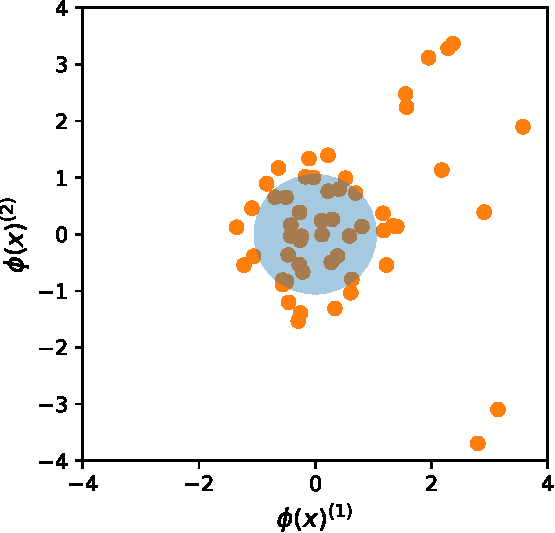
\includegraphics[scale=.65]{figure/fuzzification11.pdf}
\caption{Esempio di sfera soluzione in uno spazio bidimensionale.\label{fuzzification11}}
\end{figure}
\begin{figure}[!h]
        \centering%
       \subfigure[Fuzzificazione lineare.\label{fuzzification12}]%
          {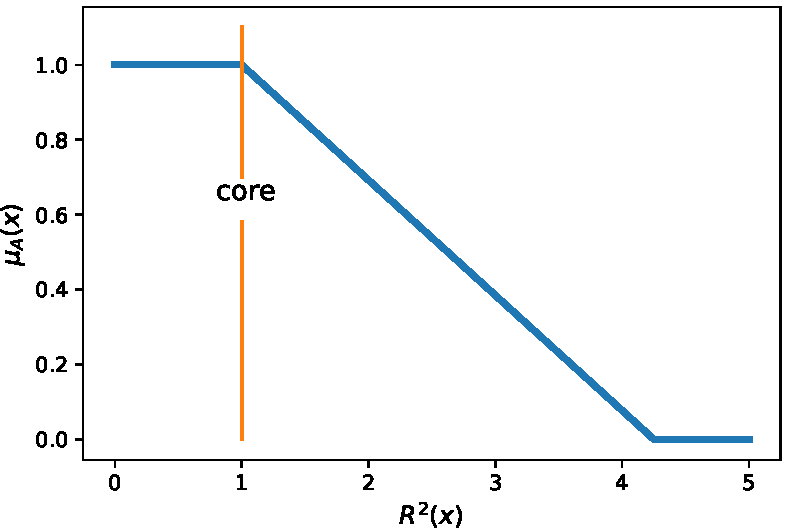
\includegraphics[scale=.4]{figure/fuzzification12.pdf}}\qquad\qquad
           \subfigure[Fuzzificazione costante a tratti, decrescente a ogni quartile.\label{fuzzification13}]%
          {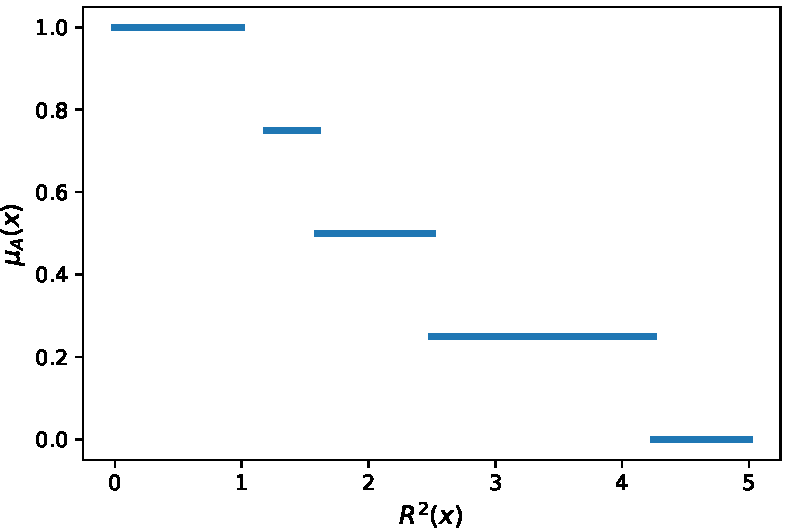
\includegraphics[scale=.4]{figure/fuzzification13.pdf}}\qquad\qquad
       \subfigure[Fuzzificazione lineare a tratti, decrescente a ogni quartile.\label{fuzzification14}]%
          {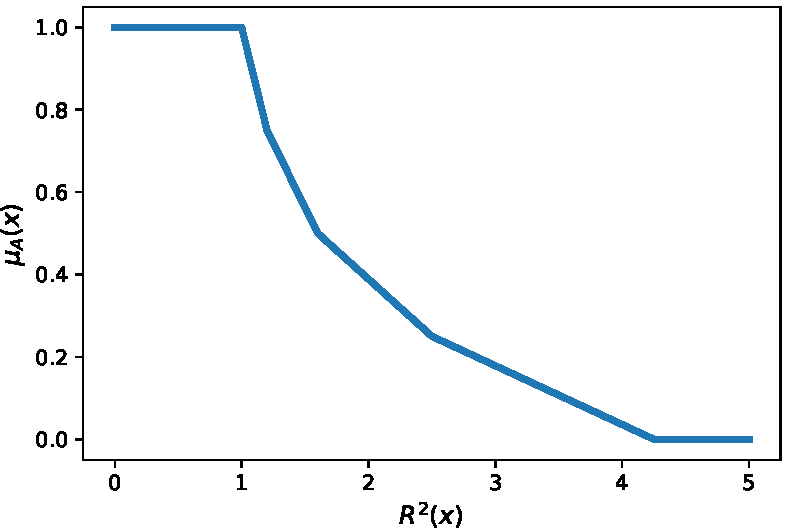
\includegraphics[scale=.4]{figure/fuzzification14.pdf}}\qquad\qquad
           \subfigure[Fuzzificazione esponenziale.\label{fuzzification15}]%
          {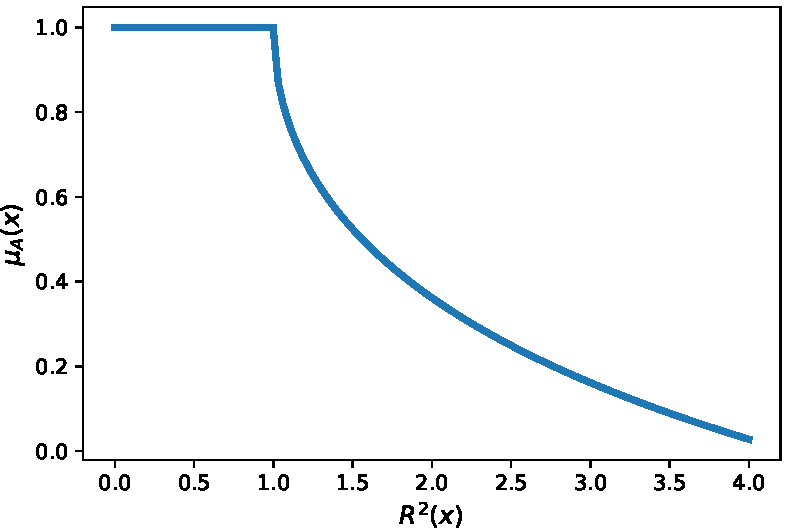
\includegraphics[scale=.4]{figure/fuzzification15.pdf}}
          \caption{Diversi esempi di fuzzificazione per l'insieme in \figurename~\ref{fuzzification11} .}
\end{figure}
\section{Costruire la funzione di appartenenza in assenza di membership: esempio con un benchmark}
Il metodo è applicabile anche in mancanza dell'insieme $U$, cioè quando il grado di membership all'insieme da apprendere è sconosciuto per i punti appartenenti al training set. Una situazione del genere è verificabile in corrispondenza di un training set del tipo definito nel Paragrafo 2.1. Il dataset Iris\cite{fisher1936use}, largamente usato nell'ambito dell'apprendimento automatico, consiste in 150 istanze del fiore Iris classificate in tre diverse specie: \textit{setosa}, \textit{virginica} e \textit{versicolor}. In base a quattro differenti feature, le tre specie si posizionano nello spazio in modo che la classe setosa sia linearmente separabile dalle altre due che invece presentano una parziale sovrapposizione. La \figurename~\ref{datasetiris} mostra il dataset nella sua rappresentazione bidimensionale dopo aver applicato la tecnica PCA\cite{abdi2010principal} di riduzione della dimensionalità.
\begin{figure}[H]
\centering
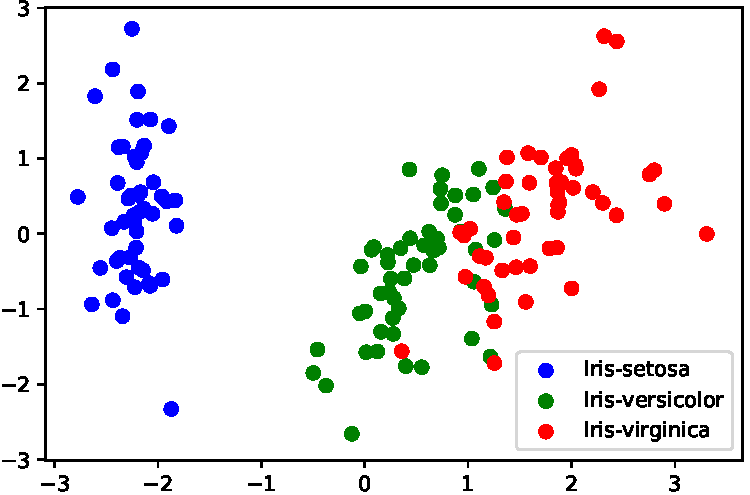
\includegraphics[scale=0.6]{figure/datasetiris.pdf}
\caption{Dataset Iris proiettato nelle sue due componenti principali. \label{datasetiris}}
\end{figure}
Supponendo di voler apprendere per una delle classi, ad esempio setosa, il corrispondente insieme fuzzy, il metodo di apprendimento appena proposto può comunque essere utilizzato costruendo l'insieme $U$ in modo tale che $\mu_i = 1$ se $x_i$ appartiene alla classe setosa, $x_i = 0$ altrimenti. Lo stesso identico ragionamento può essere applicato per le restanti classi. Ne risultano così tre funzioni di appartenenza $\mu_{setosa}$, $\mu_{virginica}$ e $\mu_{versicolor}$ apprese separatamente. Le Figure 3.3-3.5 mostrano il grafico di queste tre funzioni di appartenenza ottenute utilizzando un kernel gaussiano di parametro $\sigma$ e fissando il parametro di tradeoff $C$.
Si noti che, siccome le classi virginica e versicolor sono sovrapposte in parte e il criterio di fuzzificazione è basato sulla posizione dei punti nello spazio, i due insiemi fuzzy virginica e versicolor hanno un intersezione non vuota, come notato in \figurename~\ref{fuzzyvirginica} e in \figurename~\ref{fuzzyversicolor}. Questo significa che per alcuni punti \textit{di confine} $x_c$ risulteranno $\mu_{virginica}(x_c) > 0$ e $\mu_{versicolor}(x_c) > 0$.  Ciò non accade per l'insieme setosa che risulta disgiunto dagli altri due. Utilizzando come criterio di classificazione di un punto il grado di appartenenza maggiore al corrispettivo insieme fuzzy ne risulta un'accuratezza di previsione su punti al di fuori del training set pari a circa il 95\%.
\begin{figure}[!h]
        \centering%
        \subfigure
          {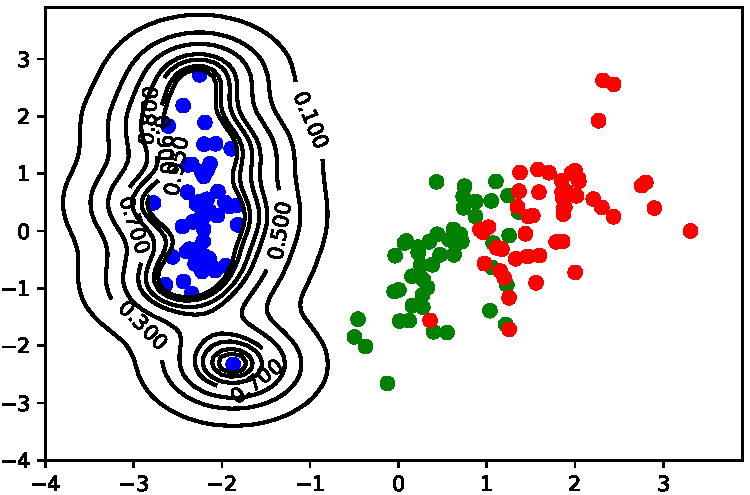
\includegraphics[scale=.5]{figure/setosamap.pdf}}\qquad\qquad
       \subfigure
          {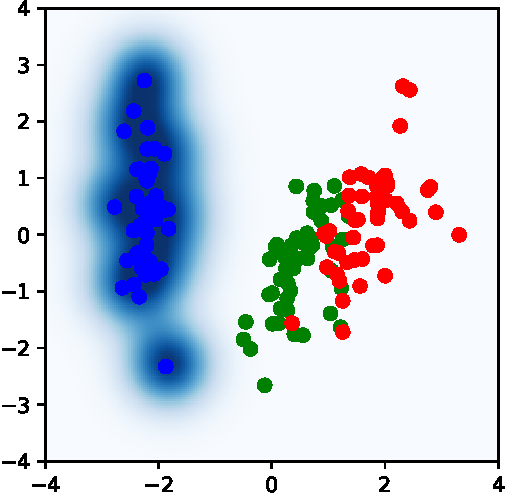
\includegraphics[scale=.5]{figure/setosaheat.pdf}}
          \caption{Contorni e mappa di calore dell'insieme fuzzy setosa. Durante l'apprendimento è stato usato il parametro $C=10$ e un kernel gaussiano di parametro $\sigma=0.5$.}
\end{figure}
\begin{figure}[!h]
        \centering%
        \subfigure
          {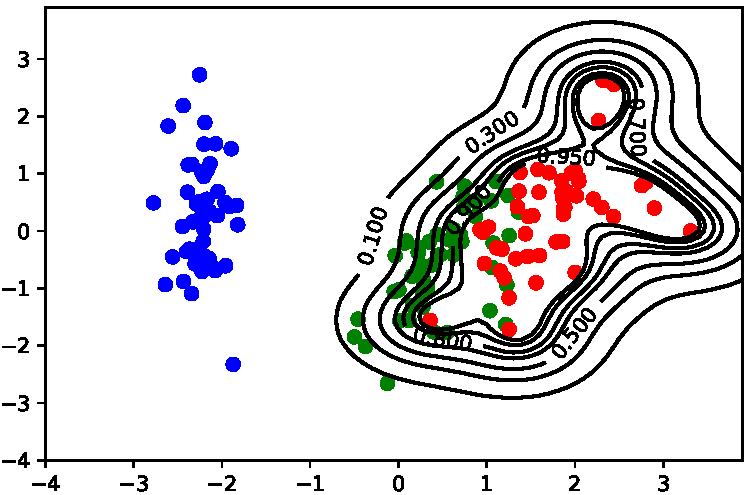
\includegraphics[scale=.5]{figure/virginicamap.pdf}}\qquad\qquad
       \subfigure
          {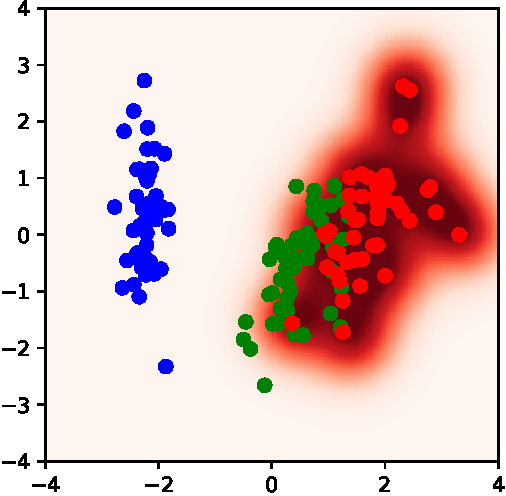
\includegraphics[scale=.5]{figure/virginicaheat.pdf}}
          \caption{Contorni e mappa di calore dell'insieme fuzzy virginica. Durante l'apprendimento è stato usato il parametro $C=10$ e un kernel gaussiano di parametro $\sigma=0.5$.\label{fuzzyvirginica}}
\end{figure}
\begin{figure}[!h]
        \centering%
        \subfigure
          {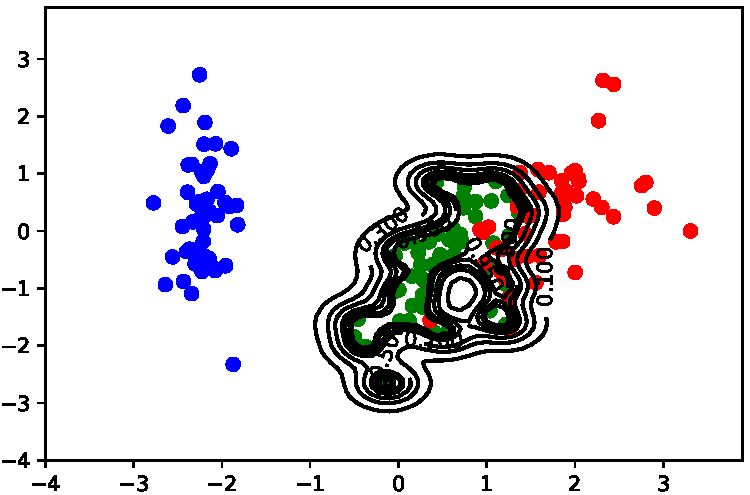
\includegraphics[scale=.5]{figure/versicolormap.pdf}}\qquad\qquad
       \subfigure
          {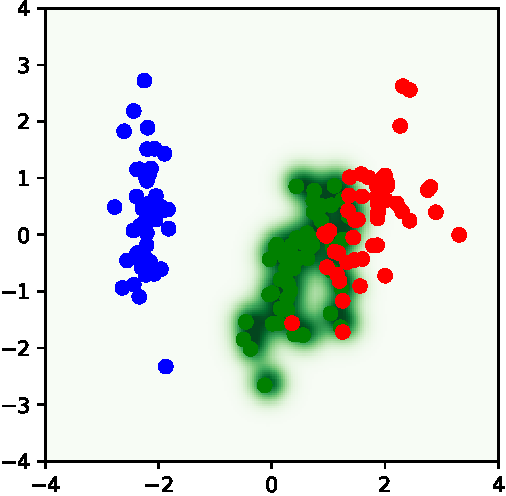
\includegraphics[scale=.5]{figure/versicolorheat.pdf}}
          \caption{Contorni e mappa di calore dell'insieme fuzzy versicolor. Durante l'apprendimento è stato usato il parametro $C=100$ e un kernel gaussiano di parametro $\sigma=0.225$.\label{fuzzyversicolor}}
\end{figure}
\chapter{Apprendimento simultaneo di insiemi fuzzy}
Il problema dell'apprendimento simultaneo di fuzzy set\cite{WIRN2018} consiste nella costruzione di un insieme $\lbrace \mu_1(\cdot), \cdots, \mu_m(\cdot) \rbrace$ di \textit{m} funzioni di appartenenza riguardanti altrettanti insiemi fuzzy $\lbrace C_1, \cdots, C_m \rbrace$. Dato un insieme di training $\lbrace x_1, \cdots, x_n \rbrace$ dove $ x_i \in X \subseteq \Omega$, $\lbrace C_1, \cdots, C_m \rbrace$ è il risultato dell'algoritmo di support vector clustering applicato all'insieme $X$ e le funzioni $\lbrace \mu_1(\cdot), \cdots, \mu_m(\cdot) \rbrace$ sono il risultato dell'algoritmo di apprendimento illustrato nel Capitolo 4 applicato a ogni $C_j$. Il problema si compone di due livelli: individuare l'insieme $\lbrace C_1, \cdots, C_m \rbrace$ e costruire le funzioni $\lbrace \mu_1(\cdot), \cdots, \mu_m(\cdot) \rbrace$.
\section{Individuazione degli insiemi fuzzy}
Il primo passo nell'individuazione dei diversi insiemi fuzzy $C_j$ è quello di costruire il problema di ottimizzazione alla base di 1-SVM per l'insieme $X$, che nella sua forma duale di Wolfe consiste nel minimizzare
\begin{equation}\label{wolfegurobi}
\sum_{i=1}^n\beta_iK(x_i,x_i) - \sum_{i=1}^n\sum_{j=1}^n\beta_i\beta_jK(x_i,x_j) 
\end{equation}
soggetta ai vincoli
\begin{equation}\label{uno}
\sum_{i=1}^n \beta_i = 1,
\end{equation}
\begin{equation}
0 \leq \beta_i \leq C \; \forall \: i \in \lbrace 1, \cdots, n\rbrace.
\end{equation}
Il valore delle soluzioni $\lbrace \beta_i^*, \cdots, \beta_n^* \rbrace$, come visto nel Paragrafo 2.2, fornisce un metodo per l'individuazione dei vettori di supporto. Vale anche in questo caso che $x_i$ è un vettore di supporto se  $0 < \beta_i^* < C.$
Una volta individuato l'insieme $S = \lbrace x_i \; | \; 0 < \beta_i < C \rbrace$ dei vettori di supporto, il quadrato del raggio della sfera di inclusione risulta essere una media tra tutti i risultati della (\refeq{r}) calcolata per ogni vettore di supporto:
\begin{equation}
R^2 = \dfrac{1}{|S|}\sum_{x \in S} R^2(x).
\end{equation}
La suddivisione in cluster viene effettuata tramite support vector clustering come descritto nel Paragrafo 2.3, ottenendo l'insieme $\lbrace C_1, \cdots, C_m \rbrace$ degli insiemi fuzzy. Per ogni insieme fuzzy trovato vale $C_j \subseteq X$. A questa prima procedura diamo il nome di \textit{procedura di primo livello}.
\section{Costruire le funzioni di appartenenza}
Le singole funzioni di appartenenza sono ottenute applicando la metodologia descritta nel Capitolo 3. Per fare ciò, è necessario ricavare per ogni futuro insieme fuzzy il grado di appartenenza $\mu_{ij}=\mu_j(x_i)$ all'insieme $C_j$ per ogni punto $x$ dell'insieme di training, cioè il corrispettivo dell'insieme $U$ nell'apprendimento di un unico fuzzy set (vedi Capitolo~\ref{malchiodi}.). Nel caso di apprendimento simultaneo l'insieme $U$ risulta essere più complesso: $U = \lbrace ( \mu_{11}, \cdots, \mu_{n1} ), \cdots, (\mu_{1m}, \cdots,  \mu_{nm})$. Per arrivare a $U$, a ogni elemento in $\lbrace C_1, \cdots, C_m \rbrace$ viene nuovamente applicato l'algoritmo di support vector clustering. Lo scopo dell'algoritmo in questo caso non è quello di suddividere l'insieme in cluster, ma quello di arrivare a conoscenza del raggio $R^2_j$ di ogni cluster $C_j$ e di ogni funzione $R_{j}^2(\cdot)$. La generica funzione $R_{j}^2(x)$ calcola il quadrato della distanza dell'immagine del generico punto $x$ dal centro del cluster $C_j$. Il raggio $R^2_j$ del cluster $C_j$ questa volta non è più calcolato come una media tra le distanze delle immagini dei vettori di supporto dal centro, ma come il massimo tra queste:
\begin{equation}
R^2_j = \max_{x \in S} [ R^2_j(x) ].
\end{equation}
La diversità nella formula del calcolo del raggio nei due diversi livelli della procedura dipende da una diversa necessità. Nel primo livello, utilizzare una media permette di avere un risultato più preciso sulla dimensione del raggio. Invece, utilizzare la media come punto di partenza per la fuzzificazione, porterebbe ad avere vettori di supporto, appartenenti al core del cluster, con un grado di appartenenza minore di uno, quando ai punti appartenenti a tale insieme è sempre assegnato il grado di appartenenza $1$.
Ottenute queste informazioni, il generico grado di appartenenza $\mu_{ij}$ è calcolato nel seguente modo:
\begin{equation}
\mu_{ij} =
\begin{cases}
1 & \text{se } R_{j}^2(x_i) \leq R^2_j, \\
\varphi(R_{j}^2(x_i)) & \text{se } R_{j}^2(x_i) > R^2_j.
\end{cases}
\end{equation}
La funzione $\varphi(\cdot)$ è un fuzzificatore qualsiasi. A questo punto è possibile applicare a ogni cluster appartenente a $\lbrace C_1, \cdots, C_m \rbrace$ la procedura di apprendimento, ottenendo l'insieme desiderato di funzioni di appartenenza $\lbrace \mu_1(\cdot), \cdots \mu_m(\cdot) \rbrace$ ai diversi insiemi fuzzy $\lbrace C_1, \cdots, C_m \rbrace$. A questa seconda procedura diamo il nome di \textit{procedura di secondo livello}.
\section{Esperimenti}
In questo capitolo viene presentato nel dettaglio l'algoritmo utilizzato per la sperimentazione della procedura di apprendimento simultaneo e i risultati ottenuti da tale sperimentazione.
\subsection{Algoritmo di validazione}
Al fine di testare la bontà dell'algoritmo di apprendimento simultaneo di insiemi fuzzy è stato costruito un sistema di validazione. In questo sistema viene iterata la ricerca di un modello ottimale tramite la prova di modelli differenti, come definito nell'Algoritmo \ref{validazione}. Per \textit{modello} si intende un insieme di funzioni di appartenenza $\lbrace \mu_1(\cdot), \cdots, \mu_m(\cdot) \rbrace$ apprese eseguendo la procedura di apprendimento simultaneo. Essendo ogni procedura dipendente dagli iperparametri $C$ e $\sigma$ indicheremo con $M_{C,\sigma}$ oppure $\lbrace \mu_1(\cdot), \cdots \mu_m(\cdot) \rbrace_{C,\sigma}$ il modello appreso tramite due specifici iperparametri. L'iperparametro $C$ corrisponde alla variabile di tradeoff del problema 1-SVM, mentre l'iperparametro $\sigma$ corrisponde al parametro del kernel gaussiano.\\
L'input del sistema di validazione è il seguente:
\begin{enumerate}
\item[1.] l'insieme $X$ sul quale applicare la procedura,
\item[2.] l'insieme $Y$ contenente le eventuali etichette assegnate ai punti contenuti in $X$,
\item[3.] un insieme di possibili parametri $C$,
\item[4.] un insieme di possibili parametri $\sigma$.
\end{enumerate}
Inoltre è possibile selezionare alcuni parametri opzionali di esecuzione che, se non specificati, assumono un valore standard:
\begin{enumerate}
\item[5.] Il numero di ripetizioni $I$,
\item[6.] Un seme, \textit{seed}, con cui inizializzare il generatore di permutazioni casuali.
\item[7.] Il numero delle componenti principali da considerarsi \textit{d}.
\item[8.] La minima dimensione di un cluster accettabile \textit{min}, come percentuale sul numero di oggetti presenti nel training set. I cluster che non raggiungono la dimensione minima non vengono trasformati in fuzzy set.
\item[9.] Il fuzzificatore $\varphi(\cdot)$ con cui assegnare i valori iniziali $\mu_{ij}$ di appartenenza in input al secondo livello.
\item[10.] Il fuzzificatore $\varphi'(\cdot)$ con cui attuare la fuzzificazione dell'insieme da apprendere.
\item[11.] Il fatto di forzare il numero di cluster a essere pari al numero di diversi valori per le etichette eventualmente presenti nel training set.
\item[12.] Il fatto di forzare tutte le eventuali etichette del training set a essere rappresentate da almeno un cluster. 
\item[13.] Usare diversi parametri $C$ e $\sigma$ per i diversi livelli della procedura \footnote{L'utilizzo di valori diversi per gli iperparametri $C$ e $\sigma$ nei due differenti livelli della procedura produce modelli dipendenti non più da una coppia di iperparametri ma da una quadrupla ($C_0, \sigma_0, C_1, \sigma_1$): la coppia $(C_0, \sigma_0)$ utilizzata nel primo livello, la coppia $(C_1,\sigma_1)$ utilizzata nel secondo. Tuttavia, i risultati ottenuti sperimentando quadruple di iperparametri non presentavano differenze sostanziali dai risultati ottenuti utilizzando coppie di iperparametri, producedo di fatto solamente un aumento del tempo impiegato per la ricerca del modello ottimale.}.
\end{enumerate}
\begin{algorithm}
\caption{Meccanismo di validazione}\label{validazione}
\begin{algorithmic}[1]
\State Proiettare l'insieme di dati nelle sue \textit{d} componenti principali.
\State Costruire le tutte le possibili combinazioni dei parametri $C$ e $\sigma$.
\State Inizializzare casualmente la variabile \textit{seed}, se non definita. 
\State \textit{i}=0
\While{$i<I$}
\State Permutare casualmente l'insieme $X$.
\State Suddividere $X$ in training set, validation set e test set.
\State \textit{best-p} = []
\State \textit{best-a} = 0
\For{ogni combinazione dei parametri $C$ e $\sigma$}
\State Apprendere simultaneamente $\lbrace \mu_1(\cdot), \cdots, \mu_m(\cdot) \rbrace$ dal training set.
\State Assegnare a ogni $\lbrace \mu_1(\cdot), \cdots, \mu_m(\cdot) \rbrace$ una tra le possibili etichette.
\State Calcolare l'accuratezza \textit{a} del modello $\lbrace \mu_1, \cdots, \mu_m \rbrace$ utilizzando il validation set.
\If{\textit{a} $>$\textit{ best-a}} \State \textit{best-p} = $(C, \sigma)$. \State \textit{best-a} $=$ \textit{a} \EndIf
\EndFor
\State Con \textit{best-p} apprendere $\lbrace \mu_1, \cdots, \mu_m \rbrace$ dal training set unito con il validation set.
\State Assegnare a ogni $\lbrace \mu_1, \cdots, \mu_m \rbrace$ un'etichetta $y_j$.
\State Calcolare l'accuratezza {$a_o$} del modello ottimale $\lbrace \mu_1(\cdot), \cdots, \mu_m(\cdot) \rbrace$ utilizzando il test set.
\State i=i+1
\EndWhile
\end{algorithmic}
\end{algorithm}
\noindent
La divisione dell'insieme $X$ in training set (80\%), validation set (10\%) e test set (10\%), viene eseguita utilizzando una permutazione casuale dei dati, diversa per ogni iterazione. La scelta di un seme per l'inizializzazione del generatore di permutazioni casuali permette la ripetizione identica di un esperimento.
Utilizzando la procedura di apprendimento simultaneo nella modalità supervisionata, ad ogni funzione di appartenenza $\mu_j(\cdot)$ viene assegnata una tra le possibili etichette contenute in $Y$. Da qui in avanti si farà riferimento all'insieme $\lbrace y_1, \cdots, y_m \rbrace$, dove la generica etichetta $y_j$ è quella assegnata alla funzione $\mu_j(\cdot)$ durante l'esecuzione supervisionata della procedura. Nello specifico, ad ogni funzione di appartenenza $\mu_j(\cdot)$ viene assegnata l'etichetta più frequente tra quelle dei punti contenute nel corrispondente cluster $C_j$.
A ogni punto del validation set vengono applicate le diverse funzioni $\mu_j(\cdot)$ e a ogni punto viene assegnata l'etichetta della funzione che restituisce il grado di appartenenza più alto. L'accuratezza $a$ di ogni diverso modello $M_{C,\sigma}$ è calcolata come il rapporto tra il numero di etichette classificate correttamente e il numero di etichette totali presenti nel validation set:
\begin{equation}
a = \dfrac{\text{\# etichette corrette}}{\text{\# etichette totali}}.
\end{equation}Il modello con il valore di accuratezza più alto viene considerato il modello ottimale. In caso di pareggio tra più modelli ne viene scelto uno casualmente.
Con gli iperparametri $C_o$ e $\sigma_o$ corrispondendi al modello ottimale $M_{C_o, \sigma_o}$ viene rieseguito l'apprendimento delle $\lbrace \mu_1(\cdot), \cdots, \mu_m(\cdot) \rbrace$ utilizzando il training set sommato al validation set e successivamente calcolata l'accuratezza $a_o$ sul test set.\\
Quando si sceglie di non forzare il numero di cluster al numero di etichette differenti contenute in $Y$, è possibile che il numero $m$ dei cluster ottenuti dal primo livello di clusterizzazione sia maggiore del numero di etichette differenti. Ne consegue che esisterà almeno una coppia di insiemi fuzzy a cui è stata assegnata la stessa etichetta. Il metodo di assegnazione di un punto del validation (test) set a un insieme fuzzy è basato sul grado di appartenenza più alto. In virtù della (\refeq{unione}), apprendendo quindi i diversi insiemi fuzzy con questa modalità, il generico cluster $C_l$ rappresentante della classe etichettata $l$ risulta essere
\begin{equation}
C_l = \bigcup_{y_i = l} C_i.
\end{equation}
Quando al contrario si sceglie di forzare l'uguaglianza tra il numero di cluster e il numero di etichette differenti, vengono mantenuti i primi $k$ cluster per grandezza e si scartano gli altri, che non vengono trasformati in insiemi fuzzy. Qualora il numero $m$ di cluster individuati è tale che $m<k$, il modello non viene considerato nella ricerca di quello ottimale. Analogamente, scegliere di forzare le differenti etichette ad essere rappresentate da almeno un insieme fuzzy fa in modo che i modelli tali per cui esiste almeno un'etichetta $l \in Y$ non presente nell'insieme $\lbrace y_1, \cdots, y_m \rbrace$ non vengano considerati.\\
Va specificato che per implementare la soluzione del problema di ottimizzazione definito da (\refeq{wolfegurobi}) è stata utilizzata la libreria Gurobi Optimizer\cite{optimization2014inc}. Il risultato di questa ottimizzazione è un vettore $\lbrace \beta_1^*, \cdots, \beta_n^* \rbrace$ i cui elementi non sono mai uguali né a zero né a $C$, sebbene il numero di vettori di supporto sia strettamente minore del numero di dati a disposizione. Al fine di ottenere una soluzione consona è stata definita una soglia $\varepsilon = 10^{-4}$ tale che se $0 < \beta_i < 0 + \varepsilon$, allora $\beta_i$ viene approssimato a zero. Analogamente se $C - \varepsilon < \beta_i < C$, allora $\beta_i$ viene approssimato a $C$. I vettori di supporto risultanti dal problema di minimizzazione risultano quindi essere quegli $x_i$ la cui corrispondente $\beta_i$ è tale  che $0 + \varepsilon < \beta_i < C -\varepsilon$.
\subsection{Risultati}
Di seguito vengono mostrati i risultati sperimentali della procedura di apprendimento simultaneo descritta nei paragrafi precedenti. Nei primi esperimenti sono stati analizzati iperparametri in un insieme delle potenze di 10: Da $10^{-2}$ a $10^2$. Successivamente, in base ai risultati ottenuti, il range è stato raffinato. In ogni esperimento è stato utilizzato il dataset Iris mostrato nel Capitolo 3.\ unitamente a un numero di ripetizioni $I=10$. Nelle Tabelle \ref{wirn}-\ref{pcm}, che riassumono i risultati ottenuti, la colonna Dim. indica il numero di componenti principali utilizzate durante l'esperimento. Le colonne Avg.\ e StDev.\ indicano rispetitvamente la media e la deviazione standard dell'accuratezza calcolata sull'insieme di training e sull'insieme di test.\\
La Tabella \ref{wirn} contiene i risultati sperimentali del confronto della procedura di apprendimento simultaneo tramite support vector clustering con l'algoritmo \textit{fuzzy c-means}\cite{bezdek1984fcm}. Questo algoritmo divide il dataset in un numero prefissato $c$ di insiemi fuzzy. Per questo esperimento l'algoritmo di apprendimento simultaneo è stato quindi forzato a ottenere $c=3$ cluster, uno per ogni diversa etichetta presente nel dataset Iris. In \figurename~\ref{fwirn} è mostrato il contorno, rappresentato come curve di livello sul grado di membership, degli insiemi fuzzy ottenuti secondo questi criteri dal metodo di apprendimento simultaneo. I risultati in Tabella \ref{wirn} sono leggermente a favore dell'algoritmo proposto.
\begin{table}[!tb]
\caption{Risultato di 10 iterazioni della procedura di apprendimento simultaneo (SVC) a confronto con l'algoritmo fuzzy c-means (FCM)\label{wirn}.}
\begin{tabular}{|c|c|c|c|c|c|c|c|c|}
\hline
& \multicolumn{4}{|c|}{SVF} & \multicolumn{4}{|c|}{FCM}\\
\cline{2-9}
& \multicolumn{2}{|c|}{Train} & \multicolumn{2}{|c|}{Test} & \multicolumn{2}{|c|}{Train} & \multicolumn{2}{|c|}{Test}\\
\hline
Dim. & Avg. & StDev. & Media & StDev. & Avg. & StDev. & Media & StDev. \\
\hline
2 & 0.82 & 0.05 & 0.8 & 0.11 & 0.83 & 0.01 & 0.80 & 0.05 \\
3 & 0.87 & 0.03 & 0.83 & 0.07 & 0.83 & 0.02 & 0.84 & 0.07 \\
4 & 0.85 & 0.05 & 0.89 & 0.09 & 0.83 & 0.01 & 0.84 & 0.08 \\
\hline
\end{tabular}
\end{table}
\begin{figure}[!tb]
        \centering%
        \subfigure[setosa]%
          {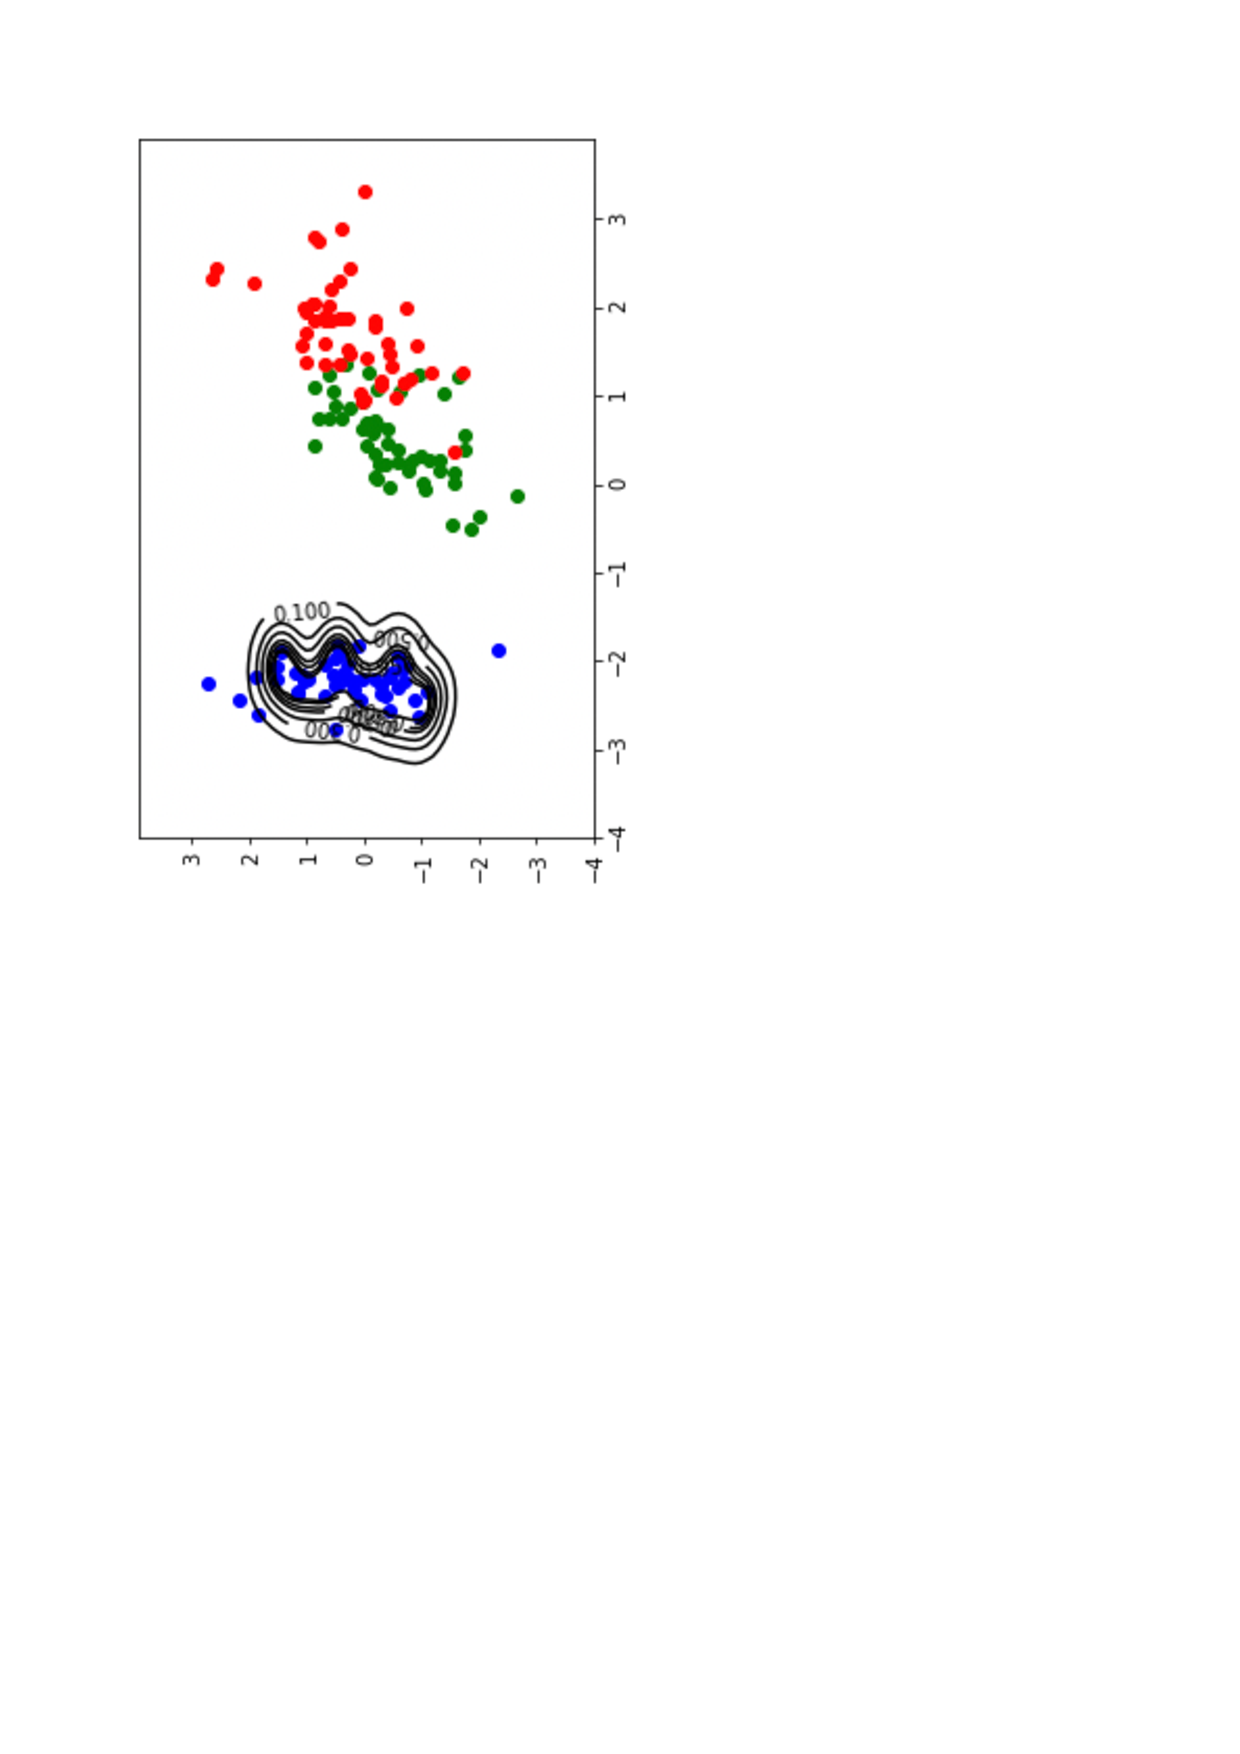
\includegraphics[scale=.35]{figure/wirnsetosa.pdf}}\qquad\qquad
       \subfigure[versicolor]%
          {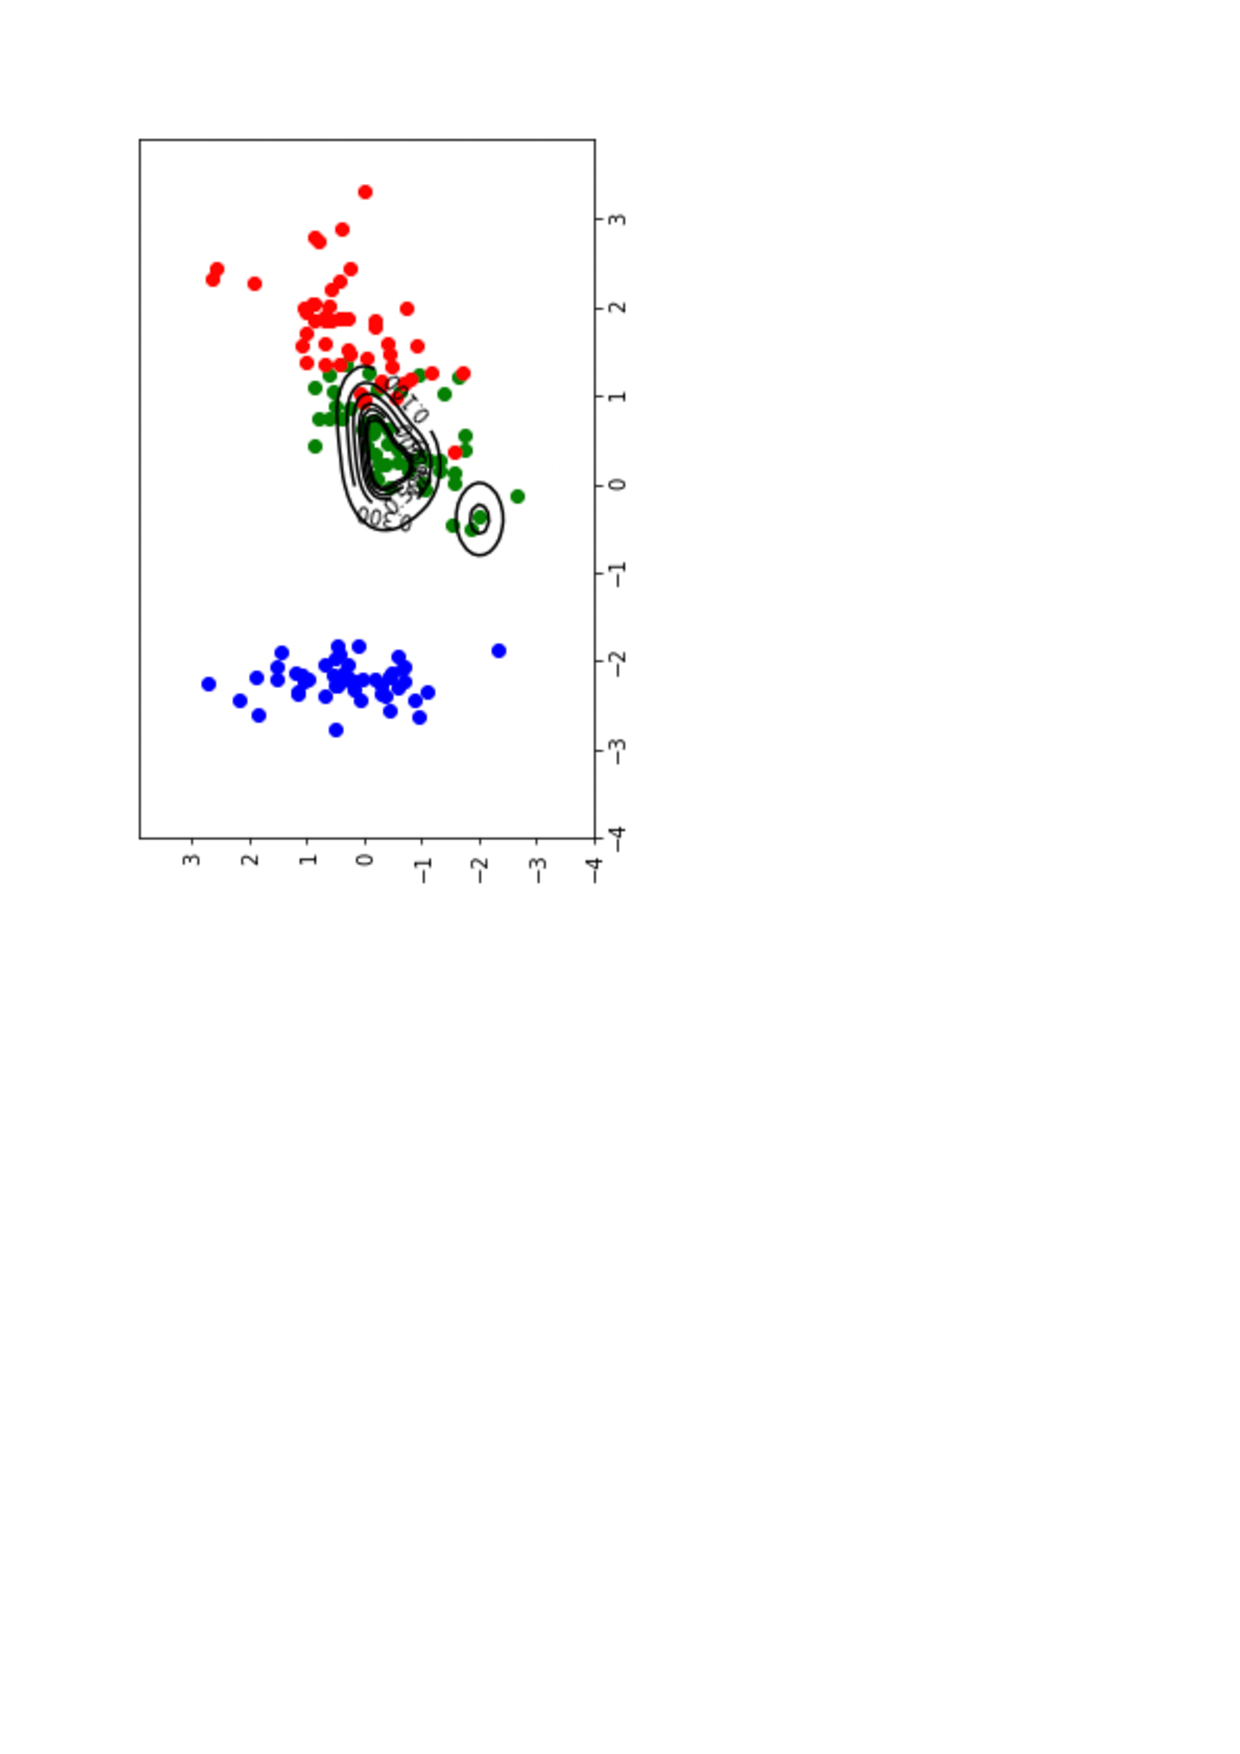
\includegraphics[scale=.35]{figure/wirnversicolor.pdf}}\qquad\qquad
           \subfigure[virginica]%
          {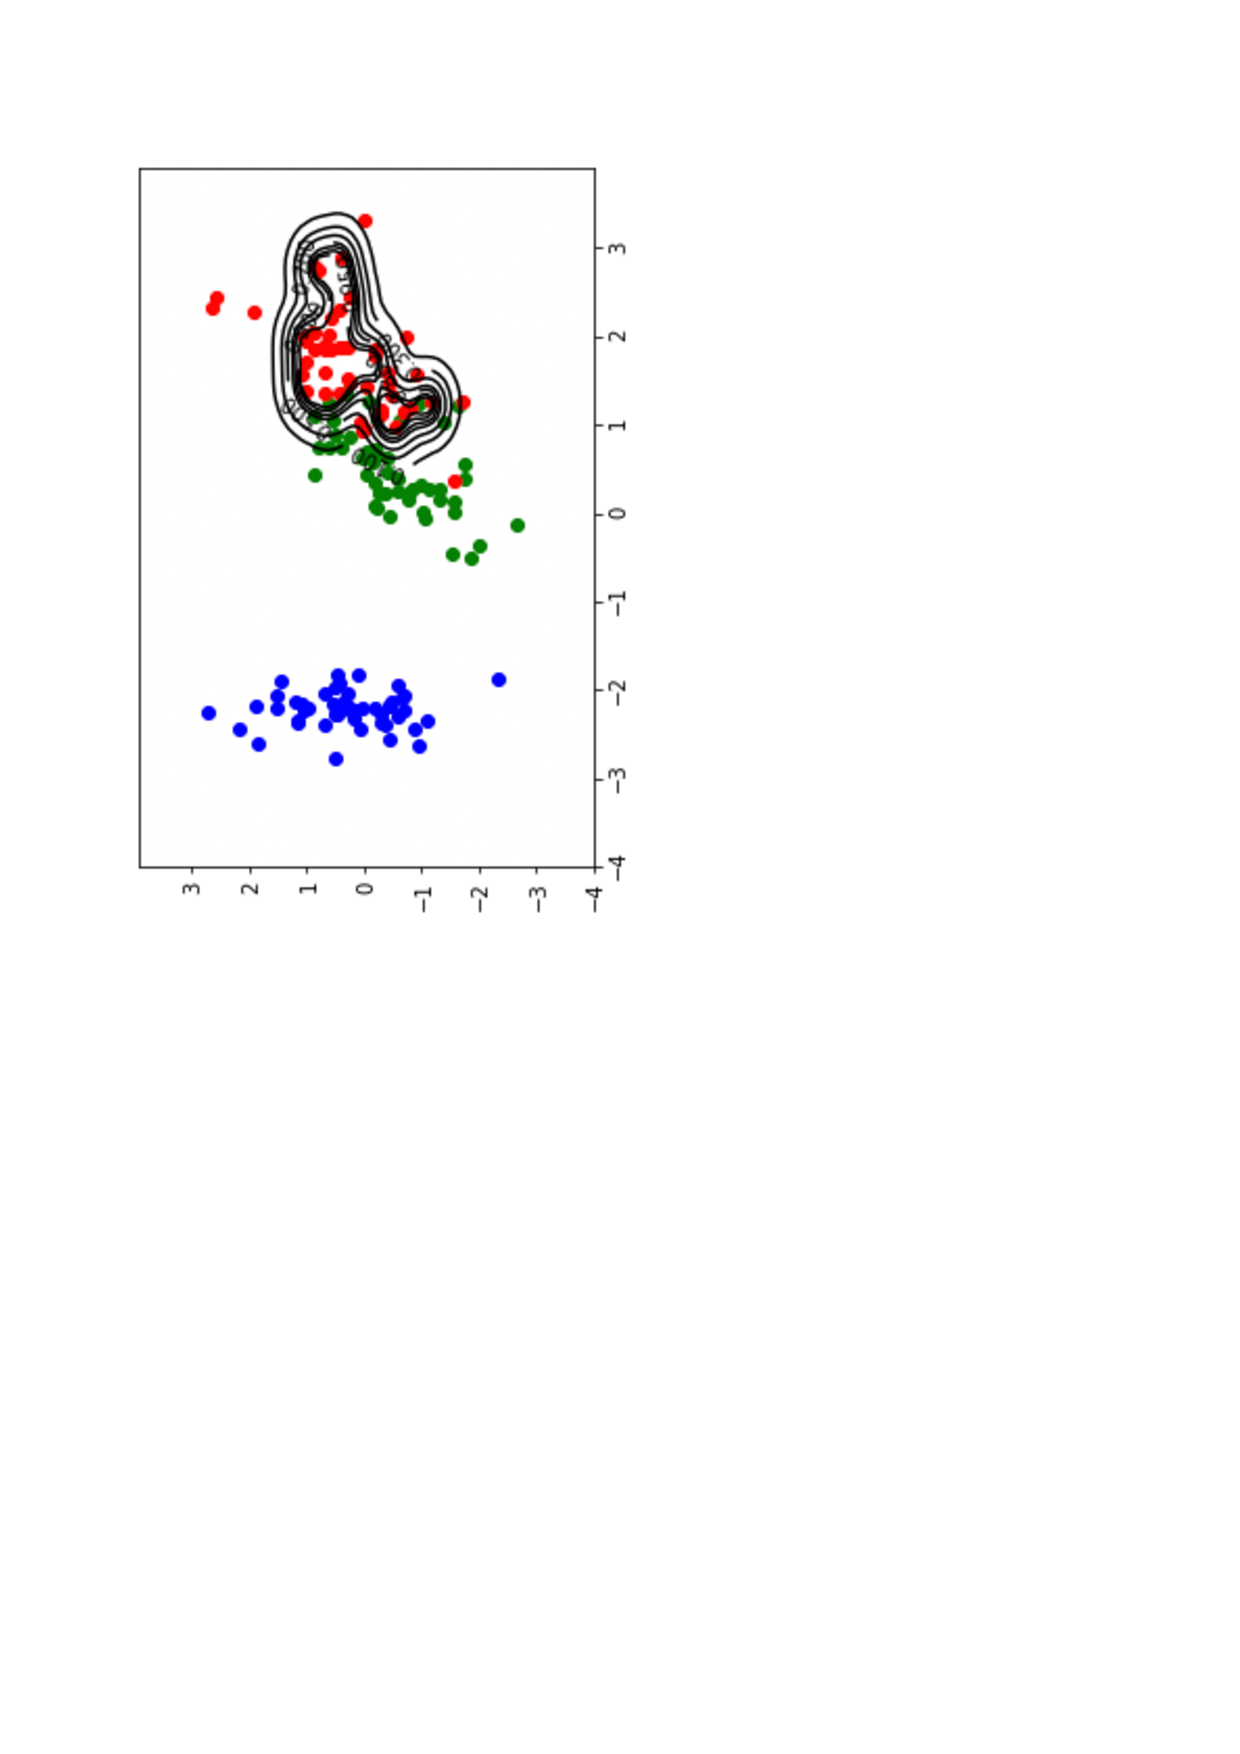
\includegraphics[scale=.35]{figure/wirnvirginica.pdf}}
          \caption{Contorno degli insiemi fuzzy setosa, versicolor e virginica\label{fwirn}.}
\end{figure}
Nella Tabella \ref{blmu} è mostrato il confronto tra l'utilizzo di membership binarie e membership linearmente decrescenti durante il clustering di secondo livello. I risultati ottenuti sono a favore delle prime. Come precedentemente notato, in presenza di $\mu_i = 0$ (\refeq{out}) tende a escludere dal core dell'insieme fuzzy il punto $x_i$. Ciò non avviene in presenza di $\mu_i > 0$. In presenza di cluster sovrapposti, l'utilizzo di gradi di appartenenza $\mu$ di tipo binario separa più facilmente i punti appartenenti a classi differenti, rendendo migliore il risultato della successiva classificazione. Va notato come l'accuratezza media calcolata nelle quattro dimensioni con $\mu$ lineari risulti sproporzionata rispetto alle altre e presenti una più alta deviazione standard. Non forzando il numero di cluster a essere uguale a quello delle etichette, da un lato si ottengono insiemi fuzzy più precisi, definiti come l'unione di insiemi più piccoli, dall'altro è possibile incorrere in modelli composti da un numero di  insiemi fuzzy minori del numero delle diverse etichette. La conseguenza di questo evento è un calo nella precisione di classificazione. Questo spiega il valore medio fuori scala e la più alta deviazione standard presenti nell'ultima riga della Tabella \ref{blmu}. Le Figure \ref{blsetosa}-\ref{blvirg} mostrano un esempio dei controni degli insiemi fuzzy ottenuti durante questa sperimentazione.
\begin{table}[!tb]
\caption{Risultato di 10 iterazioni della procedura di apprendimento simultaneo utilizzando $\mu$ di tipo binario e lineare. \label{blmu}.}
\begin{tabular}{|c|c|c|c|c|c|c|c|c|}
\hline
& \multicolumn{4}{|c|}{$\mu$ binarie} & \multicolumn{4}{|c|}{$\mu$ lineari}\\
\cline{2-9}
& \multicolumn{2}{|c|}{Train} & \multicolumn{2}{|c|}{Test} & \multicolumn{2}{|c|}{Train} & \multicolumn{2}{|c|}{Test}\\
\hline
Dim. & Avg. & StDev. & Media & StDev. & Avg. & StDev. & Media & StDev. \\
\hline
2 & 0.83 & 0.80 & 0.84 & 0.17 & 0.80 & 0.04 & 0.80 & 0.08 \\
3 & 0.90 & 0.06 & 0.88 & 0.06 & 0.84 & 0.07 & 0.84 & 0.15 \\
4 & 0.84 & 0.10 & 0.81 & 0.13 & 0.77 & 0.20 & 0.67 & 0.24 \\
\hline
\end{tabular}
\end{table}
\begin{figure}[!tb]
\centering
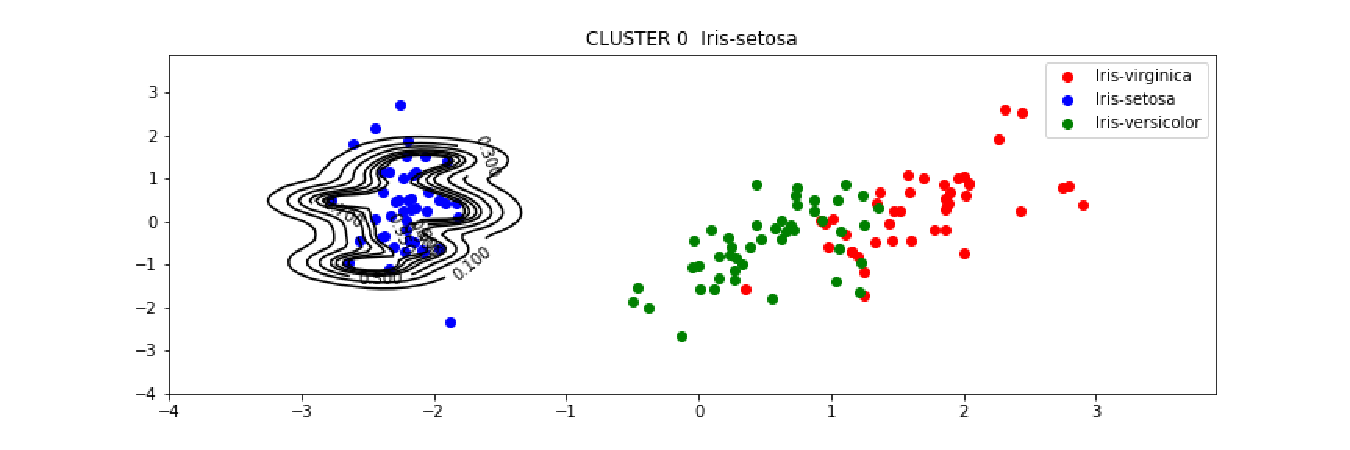
\includegraphics[scale=0.5]{figure/blset1.pdf}
\caption{Insieme fuzzy setosa appreso tramite $\mu$ binarie.\label{blsetosa}}
\end{figure}
\begin{figure}[!bt]
        \centering%
        \subfigure%
          {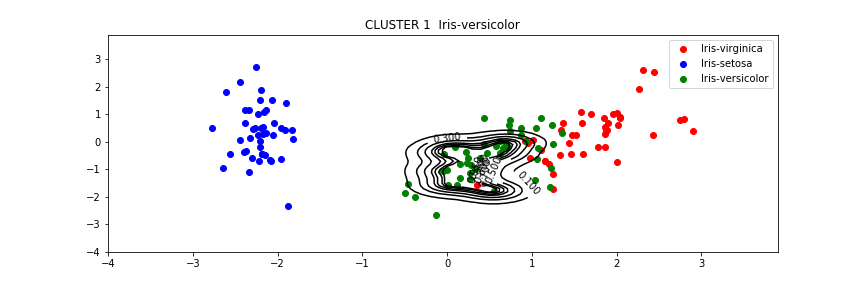
\includegraphics[scale=.3, angle=90]{figure/blvers1.png}}\qquad\qquad
       \subfigure%
          {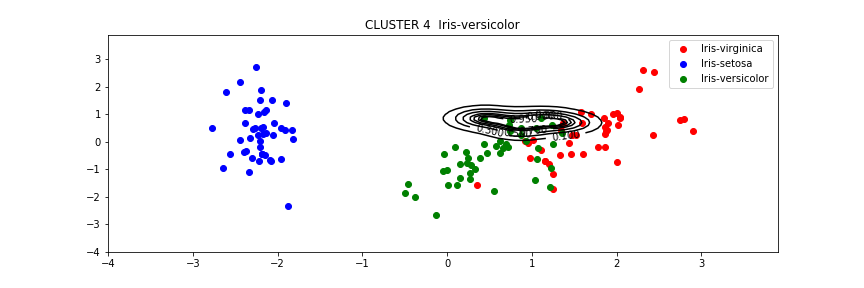
\includegraphics[scale=.3, angle=90]{figure/blvers2.png}}\qquad\qquad
           \subfigure%
          {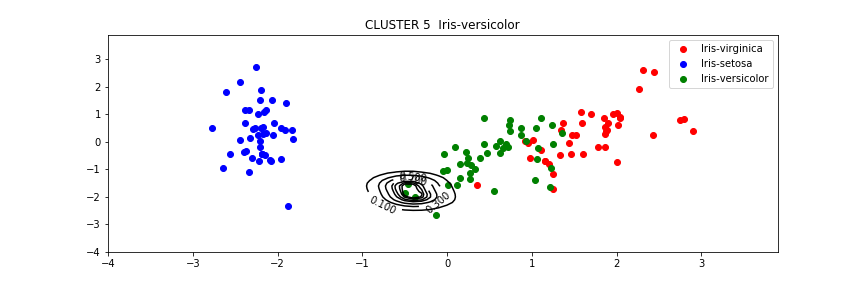
\includegraphics[scale=.3, angle= 90]{figure/blvers3.png}}
          \caption{Insieme fuzzy versicolor appreso tramite $\mu$ binarie. L'insieme risulta essere l'unione dei tre insiemi i cui contorni sono mostrati in figura.\label{blvers}.}
\end{figure}
\begin{figure}[!tb]
        \centering%
        \subfigure%
          {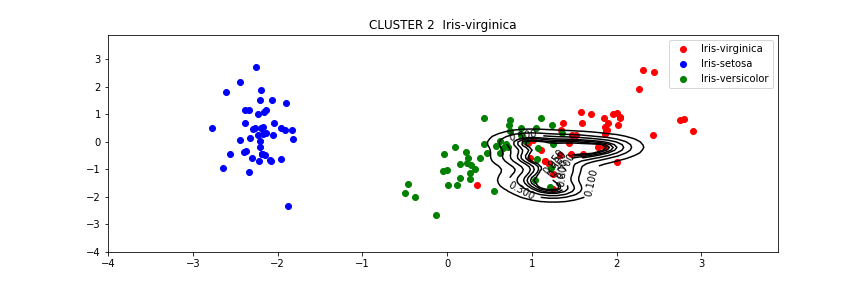
\includegraphics[scale=.3, angle=90]{figure/blvirg1.png}}\qquad\qquad
       \subfigure%
          {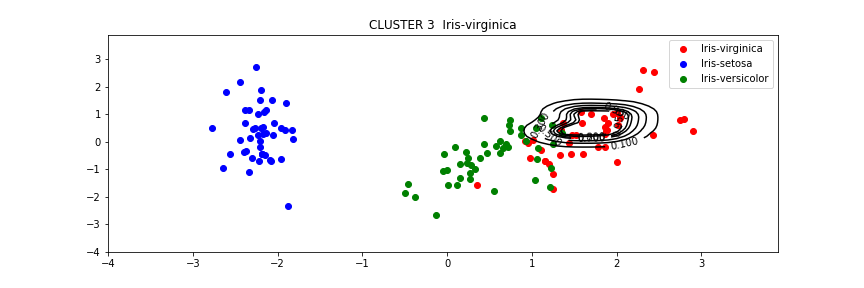
\includegraphics[scale=.3, angle=90]{figure/blvirg2.png}}\qquad\qquad
           \subfigure%
          {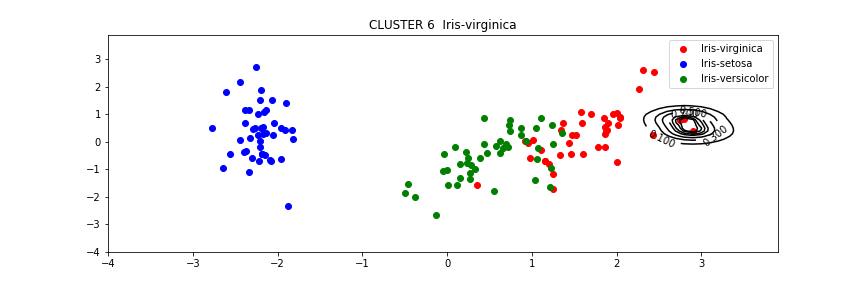
\includegraphics[scale=.3, angle=90]{figure/blvirg3.png}}
          \caption{Insieme fuzzy virginica appreso tramite $\mu$ binarie. L'insieme risulta essere l'unione dei tre insiemi i cui contorni sono mostrati in figura.\label{blvirg}.}
\end{figure}Le Tabelle \ref{df} e \ref{ef} contengono i risultati ottenuti variando il metodo di fuzzificazione tra quelli presenti in \figurename~\ref{diff}.
\begin{figure}[!tb]
        \centering%
        \subfigure[Fuzzificazione crisp.\label{fuzzification21}]%
          {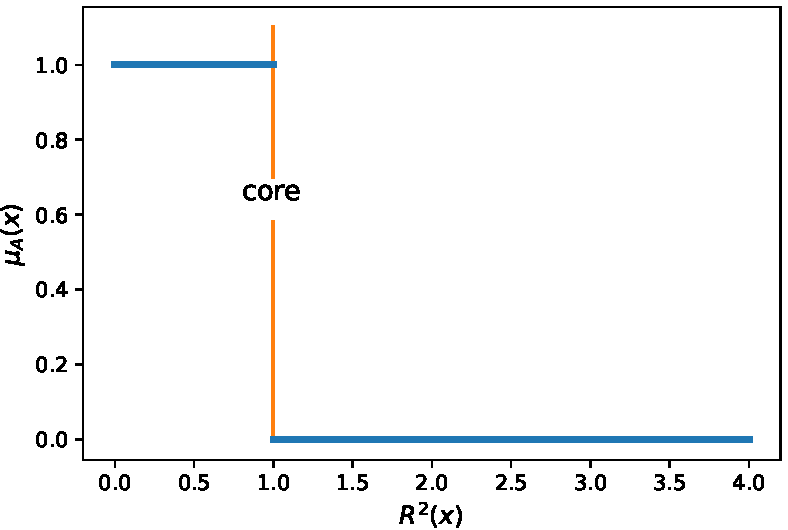
\includegraphics[scale=.4]{figure/fuzzification21.pdf}}\qquad\qquad
       \subfigure[Fuzzificazione lineare.\label{fuzzification22}]%
          {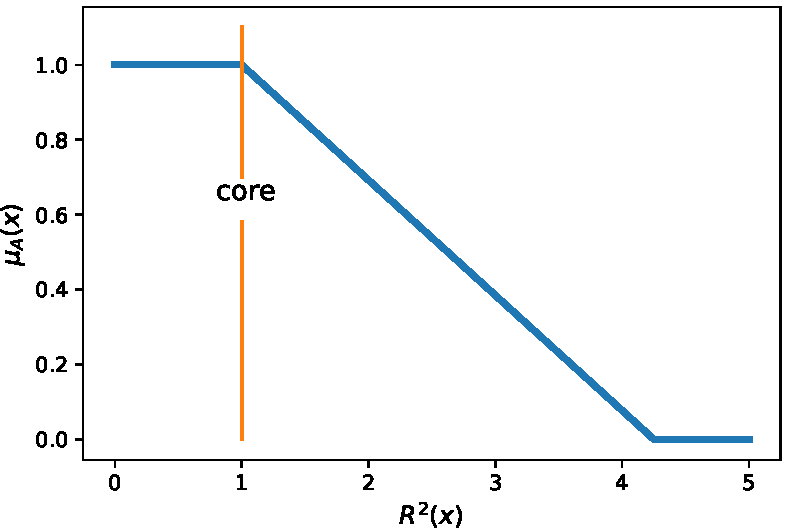
\includegraphics[scale=.4]{figure/fuzzification22.pdf}}\qquad\qquad
           \subfigure[Fuzzificazione costante a tratti, decrescente a ogni quartile (QuantCost.).\label{fuzzification23}]%
          {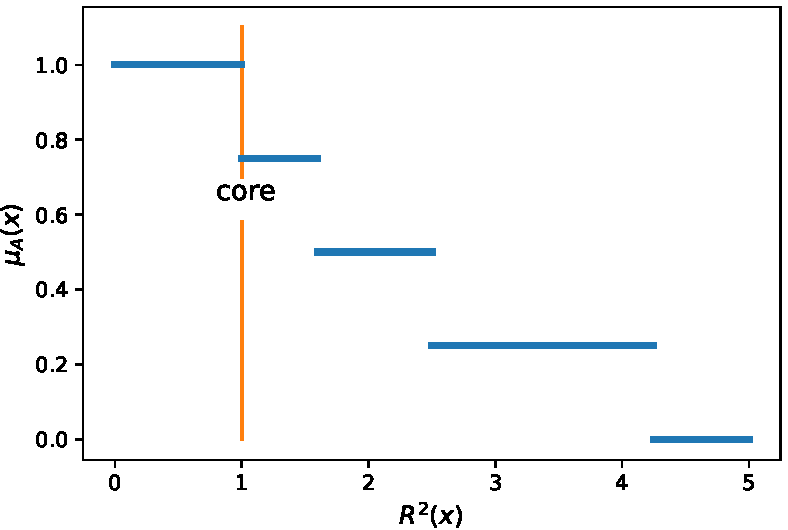
\includegraphics[scale=.4]{figure/fuzzification23.pdf}}\qquad\qquad
       \subfigure[Fuzzificazione lineare a tratti, decrescente a ogni quartile (QuantLin.).\label{fuzzification24}]%
          {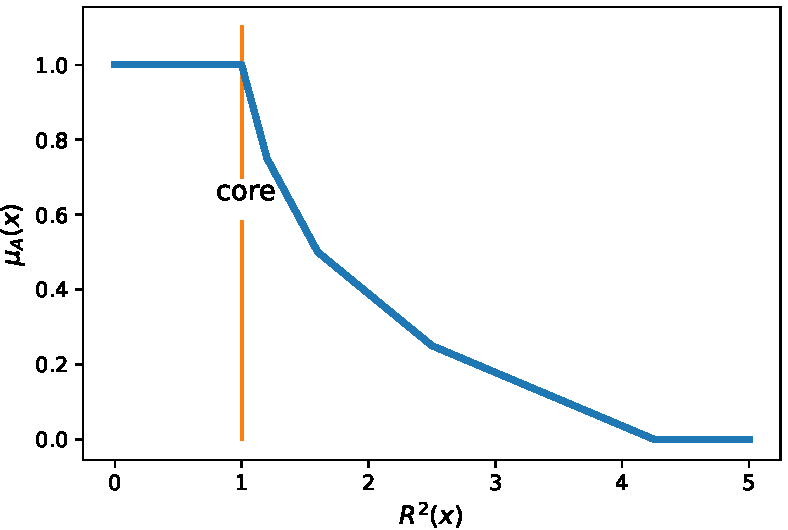
\includegraphics[scale=.4]{figure/fuzzification24.pdf}}\qquad\qquad
           \subfigure[Fuzzificazione esponenziale. Inserire descrizione parametro alfa.\label{fuzzification25}]%
          {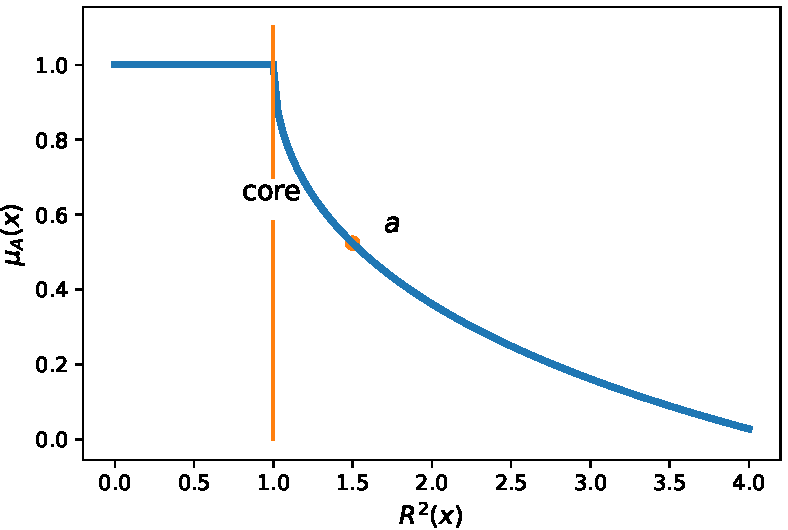
\includegraphics[scale=.4]{figure/fuzzification25.pdf}}
          \caption{Metodi di fuzzificazione.\label{diff}}
\end{figure}
\begin{table}[!tb]
\caption{Risultato di 10 iterazioni della procedura di apprendimento simultaneo utilizzando diverse funzioni decrescenti durante il processo di fuzzificazione. \label{df}.}
\begin{tabular}{|c|c|c|c|c|c|c|c|c|}
\hline
& \multicolumn{4}{|c|}{Crisp} & \multicolumn{4}{|c|}{QuantCost.}\\
\cline{2-9}
& \multicolumn{2}{|c|}{Train} & \multicolumn{2}{|c|}{Test} & \multicolumn{2}{|c|}{Train} & \multicolumn{2}{|c|}{Test}\\
\hline
Dim. & Avg. & StDev. & Media & StDev. & Avg. & StDev. & Media & StDev. \\
\hline
2 & 0.58 & 0.14 & 0.42 & 0.15 & 0.71 & 0.05 & 0.61 & 0.13 \\
3 & 0.48 & 0.07 & 0.38 & 0.14 & 0.49 & 0.11 & 0.44 & 0.16 \\
4 & 0.48 & 0.07 & 0.34 & 0.05 & 0.41 & 0.05 & 0.33 & 0.15 \\
\hline
\hline
& \multicolumn{4}{|c|}{Lineare} & \multicolumn{4}{|c|}{QuantLin.}\\
\cline{2-9}
& \multicolumn{2}{|c|}{Train} & \multicolumn{2}{|c|}{Test} & \multicolumn{2}{|c|}{Train} & \multicolumn{2}{|c|}{Test}\\
\hline
Dim. & Avg. & StDev. & Media & StDev. & Avg. & StDev. & Media & StDev. \\
\hline
2 & 0.83 & 0.80 & 0.84 & 0.17 & 0.76 & 0.10 & 0.80 & 0.15 \\
3 & 0.90 & 0.06 & 0.88 & 0.06 & 0.83 & 0.17 & 0.80 & 0.16 \\
4 & 0.84 & 0.10 & 0.81 & 0.13 & 0.70 & 0.14 & 0.70 & 0.20 \\
\hline
\end{tabular}
\end{table}
\begin{table}[!tb]
\caption{Risultato di 10 iterazioni della procedura di apprendimento simultaneo utilizzando la funzione esponenziale di parametro $\alpha$ \label{ef}.}
\begin{tabular}{|c|c|c|c|c|c|c|c|c|}
\hline
& \multicolumn{4}{|c|}{$\alpha=0.2$} & \multicolumn{4}{|c|}{$\alpha=0.4$.}\\
\cline{2-9}
& \multicolumn{2}{|c|}{Train} & \multicolumn{2}{|c|}{Test} & \multicolumn{2}{|c|}{Train} & \multicolumn{2}{|c|}{Test}\\
\hline
Dim. & Avg. & StDev. & Media & StDev. & Avg. & StDev. & Media & StDev. \\
\hline
2 & 0.82 & 0.08 & 0.75 & 0.15 & 0.80 & 0.12 & 0.80 & 0.16 \\
3 & 0.80 & 0.18 & 0.75 & 0.19 & 0.82 & 0.10 & 0.77 & 0.12 \\
4 & 0.63 & 0.0.09 & 0.56 & 0.13 & 0.55 & 0.19 & 0.44 & 0.14 \\
\hline
\hline
& \multicolumn{4}{|c|}{$\alpha=0.6$} & \multicolumn{4}{|c|}{$\alpha=0.8$.}\\
\cline{2-9}
& \multicolumn{2}{|c|}{Train} & \multicolumn{2}{|c|}{Test} & \multicolumn{2}{|c|}{Train} & \multicolumn{2}{|c|}{Test}\\
\hline
Dim. & Avg. & StDev. & Media & StDev. & Avg. & StDev. & Media & StDev. \\
\hline
2 & 0.86 & 0.05 & 0.80 & 0.12 & 0.77 & 0.19 & 0.68 & 0. 30\\
3 & 0.71 & 0.31 & 0.76 & 0.21 & 0.84 & 0.10 & 0.82 & 0.13 \\
4 & 0.63 & 0.10 & 0.60 & 0.14 & 0.60 & 0.14 & 0.52 & 0.19 \\
\hline
\end{tabular}
\end{table}I risultati peggiori si hanno in corrispondenza delle fuzzificazioni crisp e costante a tratti. Queste funzioni infatti presentano dei confini ben precisi di passaggio da un grado di membership a un altro e mal si adattano alla rappresentazione di un insieme fuzzy. Diversamente, le funzioni che decrescono in maniera continua ottengono buoni risultati. In \figurename~\ref{crispset} sono visualizzati i contorni degli insiemi fuzzy setosa, versicolor e virginica appresi mediante una fuzzificazione di tipo crisp. Da notare come, in questo caso, i confini degli insiemi risultino più evidenti che nelle altre figure proposte. In \figurename~\ref{qc} è possibile vedere la mappa di calore degli stessi insiemi fuzzy, appresi con fuzzificazione costante a tratti. Le diverse tonalità di colore che demarcano il diminuire del grado di appartenenza, anche in questo caso, si differenziano nettamente. 
\begin{figure}[!tb]
        \centering%
        \subfigure%
          {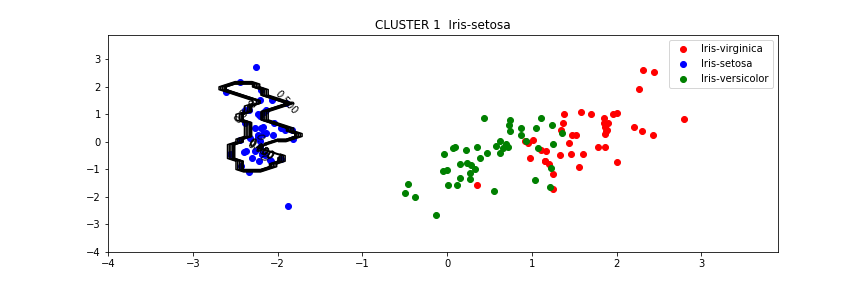
\includegraphics[scale=.3, angle=90]{figure/crispset1.png}}\qquad\qquad
       \subfigure%
          {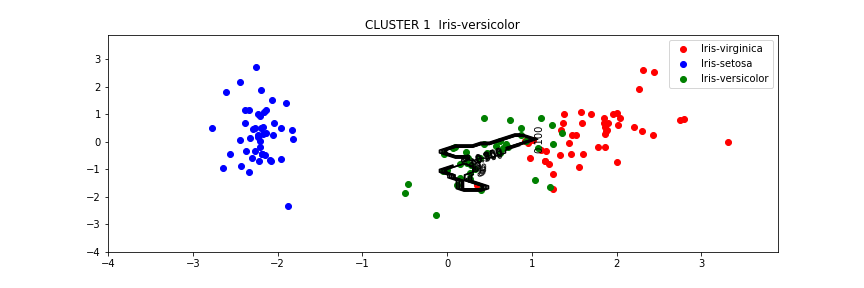
\includegraphics[scale=.3, angle=90]{figure/crispset2.png}}\qquad\qquad
           \subfigure%
          {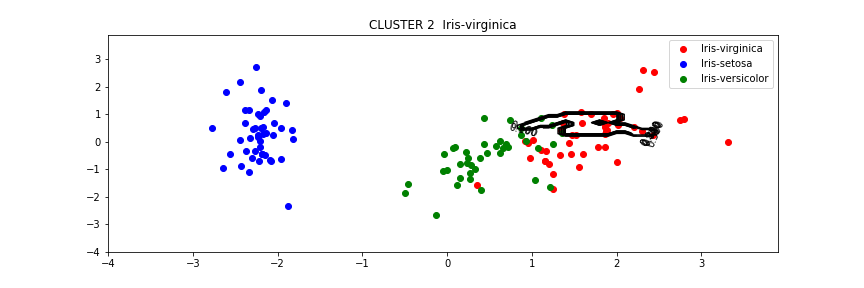
\includegraphics[scale=.3, angle=90]{figure/crispset3.png}}
          \caption{Risultato dell'apprendimento simultaneo con funzione di fuzzificazione crisp\label{crispset}.}
\end{figure}
\begin{figure}[!tb]
        \centering%
        \subfigure%
          {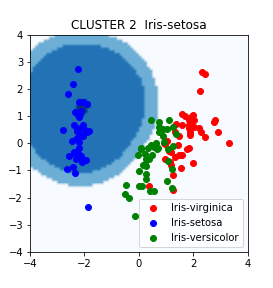
\includegraphics[scale=.3]{figure/qc1.png}}\qquad\qquad
       \subfigure%
          {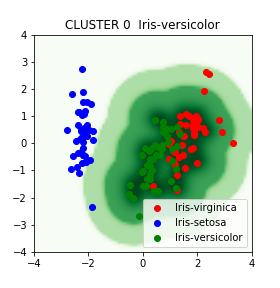
\includegraphics[scale=.3]{figure/qc2.png}}\qquad\qquad
           \subfigure%
          {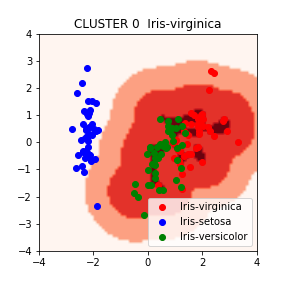
\includegraphics[scale=.3]{figure/qc3.png}}
          \caption{Mappa di calore degli insiemi fuzzy  setosa, versicolor e virginica appresi mediante una fuzzificazione di tipo costante a tratti\label{qc}.}
\end{figure}
Infine, in Tabella \ref{pcm} sono presentati i risultati ottenuti applicando l'algoritmo di clustering \textit{possibilistic c-means}\cite{filippone2010applying} in sostituzione a 1-SVM. Nel caso possibilistico i gradi di appartenenza non dipendono dalla distanza ma sono un'interpretazione probabilistica e possibilistica.
\begin{table}[!tb]
\centering%
\caption{Risultato di 10 iterazioni della procedura di apprendimento simultaneo utilizzando il metodo di clustering possibilistico\label{pcm}.}
\begin{tabular}{|c|c|c|c|c|}
\hline
& \multicolumn{2}{|c|}{Train} & \multicolumn{2}{|c|}{Test} \\
\hline
Dim. & Avg. & StDev.& Avg. & StDev. \\
\hline
2 & 0.86 & 0.03 & 0.84 & 0.12   \\
3 & 0.83 & 0.05 & 0.80 & 0.15  \\
4 & 0.82 & 0.01 & 0.84 & 0.07 \\
\hline
\end{tabular}
\end{table}
\section{Complessità}
Prendendo come riferimento l'algoritmo SMO\cite{platt1998sequential} per la risoluzione di problemi di ottimizzazione quadratici, la complessità temporale per la risoluzione del problema di ottimizzazione alla base del support vector clustering risulta, anche per l'apprendimento simultaneo di insiemi fuzzy, pari a $O(n^2)$, dove $n$ è il numero di esempi presenti nel training set. Indicando rispettivamente con $n_{sv}$ il numero di support vector individuati a valle del problema di ottimizzazione e con $n_{out}$ il numero di outlier, la complessità della fase di ricerca dei cluster, dovendo costruire e controllare le condizioni di appartenenza allo stesso cluster per ogni possibile coppia di punti, risulta essere $O((n-n_{out})^2)$. È possibile ridurre la complessità della fase di clustering controllando i segmenti congiungenti le sole coppie di punti contenenti un vettore di supporto senza perdite nell'accuratezza\cite{ben2001support}. Tale complessità risulta quindi diminuire a $O((n-n_{out})n_{sv})$. Il valore $n_{out}$ è controllato dal parametro $C$ come osservato in\cite{ben2001support} mediante la disequazione 
\begin{equation}
n_{out} < \dfrac{1}{nC}.
\end{equation}
È necessario evidenziare che questo procedimento viene applicato ulteriormente, per ogni cluster, in quello che è stato chiamato secondo livello dell'apprendimento simultaneo di fuzzy set.\\
Si noti infine che un metodo recentemente proposto, basandosi su proprietà topologiche delle funzioni kernel\cite{lee2005improved}, riduce la complessità della clusterizzazione a $O(n)$ e, in specifiche situazioni, a $O(nlog(n))$.  L'accuratezza della classificazione ne risulta però deteriorata.
\chapter*{Conclusioni}
Questa tesi ha proposto l'estensione di un metodo di apprendimento per funzioni di appartenenza a un insieme fuzzy. In particolare, l'algoritmo originale (basato sul concetto di support vector clustering) è stato adattato al fine di apprendere in modo simultaneo le funzioni di appartenenza di molteplici insiemi fuzzy definiti in uno stesso spazio. Una volta definita la procedura in maniera analitica è stato costruito un ambiente per la sperimentazione e l'analisi dell'algoritmo in modo supervisionato, al fine di testare la procedura secondo diverse opzioni. In particolare, per la fase di fuzzificazione, che risulta essere centrale nell'apprendimento di insiemi fuzzy, sono state utilizzate differenti tipologie di funzioni. I risultati sperimentali hanno mostrato come l'utilizzo di funzioni più vicine al modello di appartenenza crisp mal si adattano alla costruzione di insiemi sovrapposti, come per il caso delle classi \textit{versicolor} e \textit{virginica}, i cui confini si mischiano diventando così difficilmente delineabili. Per questo tipo di insiemi l'alternativa fuzzy risulta essere la più accurata. Inoltre, in facoltà dei risultati ottenuti dal confronto con l'algoritmo \textit{fuzzy c-means} si può affermare che il metodo proposto sia una valida alternativa nell'inferenza di insiemi fuzzy. Il processo di fuzzificazione risulta essere indipendente dal metodo di clustering utilizzato per l'individuazione dei diversi insiemi fuzzy. Questo apre molteplici possibilità di sviluppo, come lo sono il metodo migliorato per il support vector clustering e l'algoritmo possibilistico: il primo nell'ordine di diminuire la complessità computazionale della procedura,  mentre il secondo in virtù dei primi risultati sperimentali ottenuti, che superano in media quelli ottenuti tramite support vector clustering. Infine, un ulteriore sviluppo del lavoro proposto potrebbe essere quello di estendere l'algoritmo al fine di apprendere fuzzy set di tipo 2.
\bibliography{tesi.bib}
\bibliographystyle{unsrt}
\end{document}